% !TEX root = main.tex
% !TEX root = ../main.tex
\documentclass[12pt,a4paper,twoside,openany]{book}
% Version écran : chapitres sur n'importe quelle page, pas de page blanche.
% Pour la version IMPRIMÉE reliée : remettre "openright", supprimer la ligne
% ci-dessous, et remettre \cleardoublepage à la place des \clearpage du
% début de main.tex. La numérotation reste en chiffres arabes dans les deux cas.
\let\cleardoublepage\clearpage

% --- Langue et encodage ---
\usepackage[utf8]{inputenc}
\usepackage[T1]{fontenc}
\usepackage{lmodern}
\usepackage[french]{babel}
\usepackage{csquotes}

% --- Mise en page ---
\usepackage[top=2.5cm,bottom=2.5cm,inner=3cm,outer=2.5cm]{geometry}
\usepackage{setspace}
\onehalfspacing
\usepackage{microtype}
\usepackage{fancyhdr}
\usepackage[explicit]{titlesec}
\usepackage{titletoc}
\usepackage{emptypage}

% --- Couleurs (charte Al Wassit : anthracite et jaune) ---
\usepackage[table,dvipsnames]{xcolor}
\definecolor{anthracite}{HTML}{111827}
\definecolor{jauneaw}{HTML}{F5B700}
\definecolor{grisclair}{HTML}{F3F4F6}
\definecolor{griscode}{HTML}{F8F8F8}
\definecolor{rougeatodo}{HTML}{C00000}

% --- Figures, tableaux, listes ---
\usepackage{graphicx}
\graphicspath{{figures/}}
\usepackage{float}
\usepackage[font=small,labelfont=bf,labelsep=period]{caption}
\usepackage{subcaption}
\usepackage{booktabs}
\usepackage{tabularx}
\usepackage{longtable}
\usepackage{array}
\usepackage{multirow}
\usepackage{enumitem}
\setlist{itemsep=2pt,topsep=4pt}
\usepackage{tikz}
\usetikzlibrary{arrows.meta,positioning,shapes.geometric,fit,calc}
\usepackage{pdflscape}
\usepackage{adjustbox}

% --- Mathématiques / symboles ---
\usepackage{amsmath,amssymb}
\usepackage{pifont}

% --- Code source ---
\usepackage{listings}
\lstdefinelanguage{JSONx}{
  morestring=[b]",
  literate={:}{{{\color{anthracite}:}}}1,
  sensitive=false
}
\lstset{
  basicstyle=\ttfamily\footnotesize,
  backgroundcolor=\color{griscode},
  frame=single,
  rulecolor=\color{gray!50},
  breaklines=true,
  breakatwhitespace=false,
  columns=fullflexible,
  keepspaces=true,
  showstringspaces=false,
  numbers=left,
  numberstyle=\tiny\color{gray},
  numbersep=6pt,
  xleftmargin=1.2em,
  framexleftmargin=1em,
  commentstyle=\color{gray}\itshape,
  keywordstyle=\color{anthracite}\bfseries,
  stringstyle=\color{brown!80!black},
  captionpos=b,
  literate=
    {é}{{\'e}}1 {è}{{\`e}}1 {ê}{{\^e}}1 {à}{{\`a}}1 {â}{{\^a}}1
    {ç}{{\c c}}1 {î}{{\^i}}1 {ô}{{\^o}}1 {û}{{\^u}}1 {ù}{{\`u}}1
    {É}{{\'E}}1 {À}{{\`A}}1 {ï}{{\"i}}1
}
\lstdefinelanguage{JavaScriptx}{
  keywords={const,let,var,function,return,if,else,async,await,import,export,from,new,throw,try,catch,default,true,false,null,for,of},
  sensitive=true,
  morecomment=[l]{//},
  morecomment=[s]{/*}{*/},
  morestring=[b]',
  morestring=[b]",
  morestring=[b]`
}
\lstdefinelanguage{TypeScriptx}{
  language=JavaScriptx,
  morekeywords={interface,type,class,implements,readonly,private,public,inject,Injectable}
}

% --- Bibliographie ---
\lstset{literate={é}{{\'e}}1 {è}{{\`e}}1 {à}{{\`a}}1 {ç}{{\c c}}1 {ê}{{\^e}}1 {É}{{\'E}}1}

\usepackage[backend=biber,style=numeric,sorting=none,maxbibnames=4]{biblatex}
\addbibresource{bibliographie.bib}

% --- Liens (en dernier ou presque) ---
\usepackage[hidelinks,colorlinks=false,pdfusetitle,pdfencoding=auto,unicode]{hyperref}
\usepackage[nameinlink,noabbrev]{cleveref}
\usepackage{url}
\urlstyle{same}

% --- Glossaire / sigles ---
\usepackage[acronym,nomain,toc,nonumberlist,style=long3col]{glossaries-extra}

% --- Annotations de rédaction (à désactiver pour la version finale) ---
% Mettre \afficheratodotrue en \afficheratodofalse pour masquer les repères rouges.
\newif\ifafficheratodo
\afficheratodotrue
\newcommand{\todo}[1]{%
  \ifafficheratodo\textcolor{rougeatodo}{\textbf{[À COMPLÉTER : #1]}}\fi}

% Emplacement réservé pour une capture ou un schéma encore manquant.
% Usage : \figmanquante{label}{Légende}{Description précise de ce qu'il faut capturer}
\newcommand{\figmanquante}[3]{%
  \begin{figure}[htbp]
    \centering
    \fbox{\parbox{0.88\textwidth}{\centering\vspace{1.2cm}%
      \textcolor{rougeatodo}{\textbf{FIGURE À INSÉRER}}\\[4pt]
      \small #3\vspace{1.2cm}}}
    \caption{#2}\label{#1}
  \end{figure}}

% Figure standard (largeur en fraction de \textwidth)
\newcommand{\fig}[4][0.9]{%
  \begin{figure}[htbp]
    \centering
    \includegraphics[width=#1\textwidth]{#2}
    \caption{#3}\label{#4}
  \end{figure}}

% Source d'une figure ou d'un tableau
\newcommand{\source}[1]{\par\vspace{-2pt}{\footnotesize\textit{Source : #1}}\par}

% Raccourcis typographiques
\newcommand{\nom}[1]{\textsc{#1}}
\newcommand{\code}[1]{\texttt{\small #1}}
\newcommand{\route}[1]{{\small\path{#1}}}
\newcommand{\xapp}{Xapp}

% --- Titres de chapitres ---
\titleformat{\chapter}[display]
  {\normalfont\bfseries\color{anthracite}}
  {\filleft\Large\textsc{\chaptertitlename}~\Huge\thechapter}
  {10pt}
  {\titlerule[2pt]\vspace{8pt}\filleft\Huge #1}
\titlespacing*{\chapter}{0pt}{0pt}{30pt}
\titleformat{name=\chapter,numberless}[display]
  {\normalfont\bfseries\color{anthracite}}
  {}
  {0pt}
  {\titlerule[2pt]\vspace{8pt}\filleft\Huge #1}
\titleformat{\section}{\normalfont\Large\bfseries\color{anthracite}}{\thesection}{0.8em}{#1}
\titleformat{\subsection}{\normalfont\large\bfseries\color{anthracite}}{\thesubsection}{0.8em}{#1}
\titleformat{\subsubsection}{\normalfont\normalsize\bfseries\color{anthracite}}{\thesubsubsection}{0.8em}{#1}
\setcounter{secnumdepth}{3}
\setcounter{tocdepth}{2}

% --- En-têtes et pieds de page ---
\pagestyle{fancy}
\fancyhf{}
\fancyhead[LE]{\small\nouppercase{\leftmark}}
\fancyhead[RO]{\small\nouppercase{\rightmark}}
\fancyfoot[LE,RO]{\thepage}
\fancyfoot[RE,LO]{\footnotesize\titrecourt}
\renewcommand{\headrulewidth}{0.4pt}
\renewcommand{\footrulewidth}{0.2pt}
\fancypagestyle{plain}{%
  \fancyhf{}\fancyfoot[LE,RO]{\thepage}\renewcommand{\headrulewidth}{0pt}}

% --- Environnement encadré pour les définitions / remarques ---
\usepackage[most]{tcolorbox}
\newtcolorbox{remarque}[1][Remarque]{
  colback=grisclair,colframe=jauneaw,fonttitle=\bfseries,title=#1,
  boxrule=0.6pt,left=6pt,right=6pt,top=4pt,bottom=4pt,breakable}

\setlength{\parindent}{1.2em}
\setlength{\parskip}{3pt}
\raggedbottom
\frenchbsetup{StandardItemLabels=true}

% ---------------------------------------------------------------
% Informations administratives du rapport (un seul endroit à modifier)
% ---------------------------------------------------------------
\newcommand{\titrepfe}{Conception et développement d'une plateforme SaaS d'audit SEO et de visibilité dans les moteurs de recherche génératifs : \textsc{Xapp}}
\newcommand{\titrecourt}{Xapp -- Plateforme SaaS d'audit SEO et de visibilité IA}
\newcommand{\auteur}{Asma \textsc{Zgarni}}
\newcommand{\anneeuniv}{2025--2026}
\newcommand{\specialite}{\todo{spécialité}}
\newcommand{\diplome}{\todo{intitulé exact du diplôme}}
\newcommand{\encadrantacad}{Mme Mariem \textsc{Bouzouita}}
\newcommand{\encadrantent}{M. Youssef \textsc{Fessi}}
\newcommand{\organisme}{Xweb}
\newcommand{\etablissement}{ESPRIT -- École Supérieure Privée d'Ingénierie et de Technologie}
\newcommand{\datesoutenance}{\todo{date de soutenance}}
\newcommand{\urlprod}{\url{https://xapp.com.tn}}

\newacronym{api}{API}{Application Programming Interface}
\newacronym{rest}{REST}{Representational State Transfer}
\newacronym{saas}{SaaS}{Software as a Service}
\newacronym{seo}{SEO}{Search Engine Optimization}
\newacronym{aeo}{AEO}{Answer Engine Optimization}
\newacronym{geo}{GEO}{Generative Engine Optimization}
\newacronym{eeat}{E-E-A-T}{Experience, Expertise, Authoritativeness, Trustworthiness}
\newacronym{serp}{SERP}{Search Engine Results Page}
\newacronym{cwv}{CWV}{Core Web Vitals}
\newacronym{lcp}{LCP}{Largest Contentful Paint}
\newacronym{cls}{CLS}{Cumulative Layout Shift}
\newacronym{inp}{INP}{Interaction to Next Paint}
\newacronym{ttfb}{TTFB}{Time To First Byte}
\newacronym{gsc}{GSC}{Google Search Console}
\newacronym{psi}{PSI}{PageSpeed Insights}
\newacronym{rbac}{RBAC}{Role-Based Access Control}
\newacronym{jwt}{JWT}{JSON Web Token}
\newacronym{otp}{OTP}{One-Time Password}
\newacronym{orm}{ORM}{Object-Relational Mapping}
\newacronym{llm}{LLM}{Large Language Model}
\newacronym{sse}{SSE}{Server-Sent Events}
\newacronym{fifo}{FIFO}{First In, First Out}
\newacronym{ssr}{SSR}{Server-Side Rendering}
\newacronym{rtl}{RTL}{Right-To-Left}
\newacronym{i18n}{i18n}{Internationalisation}
\newacronym{tls}{TLS}{Transport Layer Security}
\newacronym{smtp}{SMTP}{Simple Mail Transfer Protocol}
\newacronym{oauth}{OAuth}{Open Authorization}
\newacronym{tts}{TTS}{Text-To-Speech}
\newacronym{stt}{STT}{Speech-To-Text}
\newacronym{vps}{VPS}{Virtual Private Server}
\newacronym{dns}{DNS}{Domain Name System}
\newacronym{cicd}{CI/CD}{Continuous Integration / Continuous Deployment}
\newacronym{uml}{UML}{Unified Modeling Language}
\newacronym{crud}{CRUD}{Create, Read, Update, Delete}
\newacronym{kb}{KB}{Knowledge Base (base de connaissances)}
\newacronym{rgpd}{RGPD}{Règlement général sur la protection des données}
\newacronym{inpdp}{INPDP}{Instance Nationale de Protection des Données Personnelles}
\newacronym{pfe}{PFE}{Projet de Fin d'Études}
\newacronym{cdc}{CDC}{Cahier des charges}
\newacronym{cors}{CORS}{Cross-Origin Resource Sharing}
\newacronym{json}{JSON}{JavaScript Object Notation}
\newacronym{html}{HTML}{HyperText Markup Language}
\newacronym{ui}{UI}{User Interface}
\newacronym{ux}{UX}{User Experience}
\newacronym{kpi}{KPI}{Key Performance Indicator}
\newacronym{pwa}{PWA}{Progressive Web App}
\newacronym{pdf}{PDF}{Portable Document Format}

\makeglossaries

\hypersetup{pdftitle={\titrecourt},pdfauthor={\auteur},pdfsubject={Rapport de Projet de Fin d'Études}}

\begin{document}

\pagenumbering{arabic}
\pagestyle{empty}
% Page de garde officielle ESPRIT (gabarit "Page Garde Rapport Stage(Fr)").
% Le fond est l'image officielle ; les champs sont superposés avec tikz.
\begin{titlepage}
\thispagestyle{empty}
\newgeometry{margin=0pt}
\begin{tikzpicture}[remember picture, overlay]
  % Fond officiel pleine page
  \node[anchor=north west, inner sep=0pt] at (current page.north west)
    {
\includegraphics[width=\paperwidth,height=\paperheight]{figures/page_garde_esprit.png}};

  % Année universitaire
  \node[anchor=west] at ([xshift=5.9cm,yshift=-4.5cm]current page.north west)
    {\sffamily\large\bfseries\color{anthracite} \anneeuniv};

  % Spécialité (complète le libellé "SPÉCIALITÉ :" imprimé sur le fond)
  \node[anchor=west] at ([xshift=10.9cm,yshift=-11.9cm]current page.north west)
    {\sffamily\Large\bfseries\color{anthracite} \specialite};

  % Sujet du rapport (zone blanche centrale)
  \node[anchor=north, text width=11.5cm, align=center]
    at ([xshift=14.6cm,yshift=-13.1cm]current page.north west)
    {\sffamily\Large\bfseries\color{anthracite} \titrepfe};

  % Logo du projet
  \node[anchor=north] at ([xshift=14.6cm,yshift=-16.9cm]current page.north west)
    {
\includegraphics[height=1.4cm,keepaspectratio]{figures/logos/logo_xapp.png}};

  % Réalisé par / Encadré par
  \node[anchor=north, align=center] at ([xshift=14.6cm,yshift=-19cm]current page.north west)
    {\sffamily\normalsize\textbf{Réalisé par :} \auteur\\[10pt]
     \sffamily\normalsize\textbf{Encadré par :}\\[4pt]
     \sffamily\small Encadrante ESPRIT : \encadrantacad\\[2pt]
     \sffamily\small Encadrant Entreprise : \encadrantent};

  % Logo de l'entreprise d'accueil dans le cadre pointillé
  \node at ([xshift=13.4cm,yshift=-24.55cm]current page.north west)
    {
\includegraphics[height=2.6cm,keepaspectratio]{figures/logos/logo_xweb.png}};
\end{tikzpicture}
\restoregeometry
\end{titlepage}

\clearpage
\chapter*{Dédicaces}
\thispagestyle{empty}
\vspace*{1cm}
\begin{center}
\textit{À mes parents,}\\[4pt]
pour leur patience, leurs sacrifices silencieux et la confiance qu'ils ont toujours placée en moi.

\vspace{1cm}
\textit{À ma famille et à mes proches,}\\[4pt]
qui ont supporté mes absences, mes soirées de débogage et mes humeurs de fin de sprint.

\vspace{1cm}
\textit{À mes amis,}\\[4pt]
pour les relectures, les encouragements et les moments qui ont rendu les semaines difficiles plus légères.

\vspace{1cm}
\todo{personnaliser la dédicace : nommer les personnes concernées, ajouter une dédicace à titre personnel si souhaité}
\end{center}

\clearpage
\chapter*{Remerciements}
\addcontentsline{toc}{chapter}{Remerciements}

Je remercie d'abord Dieu, qui m'a donné la santé et la persévérance nécessaires pour mener ce projet jusqu'à son terme.

Mes remerciements vont ensuite à mon encadrante académique, \encadrantacad, pour son suivi attentif, la clarté de ses remarques et sa disponibilité tout au long de ce stage. Ses questions m'ont obligée à justifier chaque choix de conception et ont sensiblement amélioré la qualité de ce travail.

Je tiens à exprimer ma reconnaissance à \encadrantent, mon encadrant au sein de \organisme, qui m'a confié un sujet concret, ancré dans l'activité réelle de l'agence, et qui m'a accordé la liberté technique indispensable pour le mener à bien. Les points de suivi réguliers avec lui ont permis de garder le projet aligné sur les besoins des clients de l'agence. Je remercie également toute l'équipe de \organisme{} pour son accueil et pour le temps qu'elle a consacré à m'expliquer les métiers du référencement naturel et du développement web. \todo{citer nommément les collègues de Xweb à remercier, si souhaité}

Je remercie l'ensemble du corps enseignant et de l'administration d'ESPRIT, qui m'ont transmis, durant ces années de formation, les bases techniques et méthodologiques sur lesquelles repose ce projet.

Mes remerciements s'adressent aussi aux membres du jury, qui me font l'honneur d'évaluer ce travail. J'espère que ce rapport saura leur donner une image fidèle de la démarche suivie et des difficultés rencontrées.

Enfin, merci à toutes les personnes qui, de près ou de loin, ont testé la plateforme, signalé des anomalies ou simplement encouragé ce projet.

\vspace{1cm}
\begin{flushright}
\auteur
\end{flushright}

\clearpage
\chapter*{Résumé}
\addcontentsline{toc}{chapter}{Résumé}

Ce rapport présente le travail réalisé dans le cadre de mon projet de fin d'études au sein de \organisme, agence tunisienne de conception d'applications web et de référencement naturel. Les propriétaires de sites web, en particulier les petites entreprises tunisiennes, disposent de peu de moyens pour savoir pourquoi leur site est mal positionné sur Google, et encore moins pour savoir s'il est cité par les assistants conversationnels comme ChatGPT. Les outils du marché (Semrush, Ahrefs, Screaming Frog) sont coûteux, facturés en devises, rédigés en anglais et produisent des listes de problèmes sans plan d'action.

Le projet \xapp{} répond à ce constat par une plateforme \gls{saas} qui automatise l'audit \gls{seo} d'un site (crawl multi-pages, analyse technique, sémantique et de performance, score sur 100), mesure sa visibilité dans les moteurs génératifs (scores \gls{aeo} et \gls{geo}, interrogation en direct de modèles de langage), puis transforme les résultats en un plan d'action sur quatorze jours et en une liste de corrections vérifiables automatiquement. La plateforme intègre aussi un agent conversationnel, Jannet, qui assiste les clients (support, réunion vocale) et les administrateurs (actions sur la plateforme avec journal d'annulation), ainsi que des outils de collaboration : tickets Kanban, messagerie d'équipe et notifications en temps réel.

L'application repose sur FastAPI et SQLAlchemy pour l'API, Next.js~16 et React~19 pour l'interface trilingue (français, anglais, arabe), PostgreSQL en production, et les API d'OpenAI, de Groq et de Google PageSpeed Insights. Elle est déployée sur un serveur privé virtuel derrière Nginx, avec un déploiement continu par GitHub Actions. \todo{vérifier les chiffres clés repris dans le résumé et la durée exacte du stage}

\medskip
\noindent\textbf{Mots-clés :} audit SEO, visibilité IA, AEO, GEO, SaaS, FastAPI, Next.js, modèles de langage, agent conversationnel, plan d'action.

\vspace{1.5cm}
\selectlanguage{english}
\chapter*{Abstract}
\addcontentsline{toc}{chapter}{Abstract}

This report describes the work carried out for my final-year project at \organisme, a Tunisian web development and search engine optimisation agency. Website owners, especially small Tunisian businesses, have few ways to understand why their site ranks poorly on Google, and even fewer to know whether conversational assistants such as ChatGPT mention them. Market tools (Semrush, Ahrefs, Screaming Frog) are expensive, billed in foreign currency, English-only, and they list problems without an action plan.

\xapp{} answers this with a SaaS platform that automates the SEO audit of a website (multi-page crawl, technical, semantic and performance analysis, score out of 100), measures its visibility in generative engines (AEO and GEO scores, live queries to language models), and turns the results into a fourteen-day action plan and a checklist of automatically verifiable fixes. The platform also includes a conversational agent, Jannet, that assists customers (support, voice meeting) and administrators (platform actions with an undo log), together with collaboration tools: Kanban tickets, team chat and real-time notifications.

The application uses FastAPI and SQLAlchemy, Next.js~16 and React~19 for a trilingual interface (French, English, Arabic), PostgreSQL in production, and the OpenAI, Groq and Google PageSpeed Insights APIs. It is deployed on a virtual private server behind Nginx with continuous deployment through GitHub Actions.

\medskip
\noindent\textbf{Keywords:} SEO audit, AI visibility, AEO, GEO, SaaS, FastAPI, Next.js, language models, conversational agent, action plan.
\selectlanguage{french}

\clearpage

\pagestyle{fancy}
\tableofcontents
\clearpage
\listoffigures
\clearpage
\listoftables
\clearpage
\glsaddall
\printglossary[type=\acronymtype,title={Liste des abréviations},style=long3col]

% Active la numérotation des chapitres sans réinitialiser le compteur de pages
\makeatletter\@mainmattertrue\makeatother
\chapter*{Introduction générale}
\addcontentsline{toc}{chapter}{Introduction générale}
\markboth{Introduction générale}{Introduction générale}

Pour une petite entreprise tunisienne, avoir un site web ne suffit plus. Encore faut-il que ce site soit trouvé. Pendant vingt ans, cela voulait dire apparaître dans la première page de Google ; aujourd'hui, une part croissante des internautes pose directement sa question à un assistant conversationnel comme ChatGPT, Perplexity ou Gemini, qui répond par un texte de synthèse et ne cite que quelques sources. Un site peut donc être bien référencé au sens classique et rester invisible dans ces nouvelles réponses. \todo{ajouter une statistique sourcée et datée sur la part des recherches passant par les assistants IA, ou supprimer cette phrase}

C'est dans ce contexte que s'inscrit mon stage chez \organisme, agence tunisienne de conception d'applications web et de référencement naturel. Une partie du travail de l'agence consiste à auditer les sites de ses clients : vérifier les balises, la structure, la vitesse, l'indexation, puis rédiger des recommandations. Ce travail est long, répétitif, et il repose sur des outils étrangers coûteux qui ne disent rien de la visibilité d'un site dans les moteurs génératifs.

Mon projet de fin d'études consiste à automatiser ce travail dans une plateforme \gls{saas}, \xapp{} (aussi appelée SEOtunisie au début du projet). Un utilisateur y saisit l'adresse de son site ; la plateforme parcourt ses pages, calcule un score \gls{seo} détaillé, évalue sa visibilité dans les moteurs de réponse (\gls{aeo}) et génératifs (\gls{geo}), interroge en direct des modèles de langage pour vérifier s'ils citent le site, puis produit un plan d'action sur quatorze jours et une liste de corrections que la plateforme sait revérifier. Autour de ce cœur, \xapp{} propose un assistant conversationnel (Jannet), un support par tickets, une messagerie d'équipe, un système de crédits et une console d'administration, dans une interface disponible en français, en anglais et en arabe.

Ce projet pose des questions techniques qui dépassent une application de gestion classique : parcourir un site inconnu sans le surcharger ni dépasser les délais d'un serveur mandataire, exécuter des traitements longs en arrière-plan, définir des scores reproductibles, et orchestrer des modèles de langage dont les réponses ne sont ni gratuites, ni déterministes, ni toujours disponibles.

Ce rapport retrace la démarche suivie, du cadrage à la mise en production. Il comprend huit chapitres :
\begin{itemize}
  \item le \textbf{premier chapitre} présente l'organisme d'accueil, analyse l'existant, formule la problématique et justifie la méthodologie retenue ;
  \item le \textbf{deuxième chapitre} est consacré à l'analyse des besoins : acteurs, exigences fonctionnelles et non fonctionnelles, cas d'utilisation, backlog et planification ;
  \item le \textbf{troisième chapitre} expose la conception : choix technologiques, architecture logique et physique, modèle de données et diagrammes de séquence de l'audit ;
  \item les \textbf{chapitres quatre à sept} détaillent la réalisation sprint par sprint : socle, comptes et contrôle d'accès, moteur d'audit SEO, visibilité IA et plan d'action, puis l'agent Jannet, la collaboration et la monétisation ;
  \item le \textbf{huitième chapitre} traite du déploiement, de la sécurité, de la validation et des limites actuelles de la solution.
\end{itemize}

Une conclusion générale dresse enfin le bilan du projet, ce qu'il m'a apporté et les évolutions envisagées.

\chapter{Contexte général du projet}

\section{Introduction}
Ce premier chapitre situe le projet. Nous commençons par présenter \organisme, où le stage s'est déroulé, puis nous décrivons la manière dont un audit de référencement est réalisé aujourd'hui et les limites des outils disponibles. Nous en déduisons la problématique et la solution retenue. Le chapitre se termine par la méthodologie de conduite de projet et les raisons qui nous ont conduite à la choisir.

\section{Présentation de l'organisme d'accueil}

\subsection{Présentation générale}
\organisme{} (Xweb Tunisie) est une agence tunisienne spécialisée dans la conception d'applications web et de solutions \gls{saas} sur mesure, l'expérience utilisateur et le référencement naturel. Sa signature, « \textit{Code. Optimize. Dominate.} », résume son positionnement : développer des plateformes performantes, les optimiser pour les moteurs de recherche, et aider ses clients à gagner en visibilité. \todo{année de création, forme juridique, adresse, effectif, à confirmer auprès de l'encadrant}

\begin{figure}[htbp]
  \centering
  
\includegraphics[width=0.25\textwidth]{figures/logos/logo_xweb.png}
  \caption{Logo de \organisme}\label{fig-logo-xweb}
\end{figure}

\fig[0.95]{figures/divers/xweb_site.png}{Page d'accueil du site institutionnel de \organisme{} et références clientes}{fig-xweb-site}
\source{capture du site web de l'agence, consultée lors du stage}

\subsection{Activités et clientèle}
L'agence intervient sur trois métiers complémentaires : le développement d'applications web et de plateformes métier, la conception d'interfaces centrées sur l'utilisateur, et l'optimisation du référencement (audit, contenu, performance). Ses clients sont majoritairement des entreprises tunisiennes de petite et moyenne taille, dont certaines figurent sur la \cref{fig-xweb-site}. \todo{vérifier avec l'agence la répartition réelle des activités et l'autorisation de publier les logos clients visibles sur la capture}

\subsection{Organisation interne}
\todo{insérer l'organigramme de l'agence (direction, développement, design, SEO, commercial) ou le décrire en quelques lignes, après validation par l'encadrant ; si l'agence ne souhaite pas le publier, supprimer cette sous-section}

\subsection{Cadre du stage}
Le stage s'inscrit dans le projet de fin d'études de la formation suivie à \etablissement. Le sujet a été formalisé dans un cahier des charges interne décrivant une plateforme d'audit \gls{seo} et de visibilité IA, ses modules fonctionnels, son architecture cible et sa feuille de route. Le projet a d'abord porté le nom de travail « SEOtunisie » ; l'application a ensuite été renommée \xapp{} pour s'aligner sur l'identité de l'agence. Elle est publiée sous le domaine \urlprod.

Le travail est encadré sur deux plans : \encadrantacad{} assure le suivi académique et \encadrantent{} le suivi technique et métier au sein de l'agence, avec des points réguliers pour valider l'orientation prise. \todo{préciser la fréquence réelle des points de suivi}

\section{Étude de l'existant}

\subsection{Description de l'existant}
Avant le projet, un audit de référencement reposait sur la combinaison de plusieurs pratiques et outils (\cref{fig-outils-existants}) :
\begin{itemize}
  \item un \textbf{audit manuel} par un consultant ou un freelance, qui inspecte les pages, relève les balises manquantes et rédige un rapport sous forme de document ;
  \item des \textbf{suites SEO commerciales} comme Semrush ou Ahrefs, qui fournissent des audits de site, des données de mots-clés et de liens entrants, sur abonnement mensuel ;
  \item des \textbf{crawlers de bureau} comme Screaming Frog SEO Spider, qui parcourent un site et listent les erreurs techniques ;
  \item des \textbf{outils gratuits de Google}, principalement PageSpeed Insights pour la performance et Google Search Console pour l'indexation.
\end{itemize}

\fig[0.7]{figures/divers/outils_existants.png}{Principaux outils d'audit SEO utilisés ou envisagés avant le projet}{fig-outils-existants}
\source{logos des éditeurs concernés ; montage réalisé pour la présentation du projet}

\subsection{Critique de l'existant}
Ces solutions sont reconnues, mais elles répondent mal aux besoins des clients de l'agence. Nous en avons retenu cinq limites, issues de l'observation du travail de l'équipe et des échanges avec l'encadrant :

\begin{description}[leftmargin=1.2em,style=nextline]
  \item[Coût et facturation en devises.] Les suites commerciales sont facturées par abonnement mensuel, de l'ordre d'une centaine de dollars par mois pour les premières offres, et payables en devises étrangères, ce qui est un frein réel pour une petite entreprise tunisienne. \todo{citer un tarif public vérifié de Semrush et d'Ahrefs, consulté à une date précise}
  \item[Diagnostic sans plan d'action.] Les rapports listent des centaines d'anomalies, souvent en termes techniques, sans dire par où commencer ni comment corriger. Le propriétaire du site reste seul face à la liste.
  \item[Aucune mesure de la visibilité IA.] Aucun de ces outils, à la date de l'étude, ne mesurait de manière simple si un site est cité par les assistants conversationnels ni s'il est structuré pour l'être (FAQ, données structurées, signaux de crédibilité). \todo{vérifier cette affirmation à la date de la soutenance : certains éditeurs ont commencé à proposer des modules de suivi IA}
  \item[Barrière de la langue.] Les interfaces sont en anglais, rarement en français et jamais en arabe, alors qu'une grande partie de la clientèle visée est arabophone ou francophone.
  \item[Suivi des corrections inexistant.] Une fois l'audit livré, rien ne permet de vérifier qu'une anomalie a été corrigée, sinon relancer un audit complet et comparer à la main.
\end{description}

Le \cref{tab-comparatif-outils} résume cette comparaison.

\begin{table}[htbp]
\centering
\small
\caption{Comparaison de l'existant avec les besoins identifiés}\label{tab-comparatif-outils}
\begin{tabularx}{\textwidth}{@{}lXXXX@{}}
\toprule
\textbf{Besoin} & \textbf{Audit manuel} & \textbf{Semrush / Ahrefs} & \textbf{Screaming Frog / PSI} & \textbf{Cible \xapp}\\
\midrule
Audit technique automatisé & Non & Oui & Oui & Oui\\
Score global compréhensible & Variable & Oui & Non & Oui\\
Plan d'action priorisé & Oui (coûteux) & Partiel & Non & Oui (IA)\\
Mesure de la visibilité IA & Non & \todo{à vérifier} & Non & Oui\\
Suivi des corrections & Non & Partiel & Non & Oui\\
Interface FR / AR & Oui & Non & Non & Oui\\
Paiement local en dinars & Oui & Non & Non & Oui\\
\bottomrule
\end{tabularx}
\end{table}

\subsection{Problématique}
De cette analyse découle la question à laquelle le projet doit répondre :

\begin{remarque}[Problématique]
Comment automatiser l'audit SEO d'un site et mesurer sa visibilité à la fois dans les moteurs de recherche classiques et dans les moteurs génératifs, tout en fournissant des recommandations actionnables et un plan d'optimisation personnalisé, à un coût accessible pour une petite entreprise tunisienne ?
\end{remarque}

Cette question en contient plusieurs. Il faut un moteur capable de parcourir un site inconnu, rapidement et sans le surcharger. Il faut des scores reproductibles, qui ne flattent pas l'utilisateur. Il faut interroger des modèles de langage externes, payants et parfois indisponibles, et transformer leurs réponses en indicateurs. Il faut enfin un modèle économique (crédits, paiement local) et une interface trilingue.

\subsection{Solution proposée}
Nous proposons \xapp, une plateforme web accessible depuis un navigateur, sans installation, organisée autour de cinq modules :
\begin{itemize}
  \item un \textbf{moteur d'audit SEO} qui parcourt jusqu'à une centaine de pages, analyse les aspects techniques, sémantiques et de performance, et calcule un score sur 100 détaillé par catégorie ;
  \item un module de \textbf{visibilité IA en direct}, qui calcule des scores AEO et GEO et interroge des modèles de langage (ChatGPT, Groq) pour savoir s'ils citent le site et ses concurrents ;
  \item un \textbf{plan d'action et un suivi des corrections}, avec un calendrier de quatorze jours généré par IA, des contenus prêts à copier et une liste de corrections revérifiables ;
  \item un \textbf{agent IA, Jannet}, qui répond aux clients, crée des tickets, anime une réunion vocale autour de l'audit et exécute des actions d'administration ;
  \item un ensemble d'outils de \textbf{collaboration et de gestion} : tickets Kanban, messagerie d'équipe, notifications, crédits, packs et console d'administration.
\end{itemize}

Les objectifs mesurables que nous nous sommes fixés sont les suivants : produire un audit complet sans intervention humaine, fournir pour chaque audit une liste de corrections priorisée et un plan d'action, permettre à l'utilisateur de vérifier une correction sans relancer d'audit complet, et proposer l'ensemble dans les trois langues de la clientèle. \todo{faire valider ces objectifs par l'encadrant}

\section{Méthodologie de conduite du projet}

\subsection{Méthodes de gestion de projet}
Avant de choisir, nous avons comparé les principales approches envisageables pour un développement de cette taille mené par une seule personne. Le \cref{tab-methodologies} en donne une synthèse.

\begin{table}[htbp]
\centering
\small
\caption{Comparaison des approches de gestion de projet envisagées}\label{tab-methodologies}
\begin{tabularx}{\textwidth}{@{}lXXX@{}}
\toprule
\textbf{Approche} & \textbf{Principe} & \textbf{Avantages} & \textbf{Limites pour ce projet}\\
\midrule
Cycle en cascade (V) & Phases séquentielles : spécification, conception, développement, test & Documentation complète, planning lisible & Les besoins évoluent en cours de route ; un retour tardif coûte cher\\
Scrum & Itérations courtes (sprints), backlog priorisé, revues et rétrospectives \cite{scrumguide} & Adaptation aux changements, livraisons régulières & Prévu pour une équipe ; certains rôles et cérémonies doivent être allégés\\
Kanban & Flux continu, limitation du travail en cours \cite{anderson2010kanban} & Très souple, adapté à la maintenance & Peu de cadence imposée, risque de dispersion\\
\bottomrule
\end{tabularx}
\end{table}

\subsection{Choix de la méthodologie}
Nous avons retenu une démarche \textbf{itérative inspirée de Scrum}. Ce choix s'explique par trois raisons.

La première est l'incertitude du domaine. La visibilité dans les moteurs génératifs est un sujet récent, sans méthode de mesure établie ; les indicateurs AEO et GEO ont été affinés au fil des retours de l'encadrant et des essais sur des sites réels. Fonctionner par itérations permettait de revoir ces choix à chaque point de suivi.

La deuxième est la nature du travail. Une développeuse unique n'a ni équipe à coordonner ni \textit{Product Owner} distinct. Nous avons donc conservé de Scrum ce qui structure le travail (backlog priorisé, sprints à objectif clair, rétrospective) et laissé de côté ce qui suppose plusieurs personnes. L'encadrant en entreprise a joué le rôle de représentant du métier, en validant l'objectif de chaque sprint et en testant les livraisons.

La troisième est la livraison continue. L'application a été déployée sur le serveur de production dès les premières semaines, et chaque fonctionnalité terminée y a été publiée automatiquement par GitHub Actions. Cela a permis de tester la plateforme sur de vrais sites, avec les vraies contraintes de réseau.

Nous avons organisé la réalisation en quatre sprints, précédés d'un sprint~0 d'analyse et de conception :

\begin{table}[htbp]
\centering
\small
\caption{Découpage du projet en sprints}\label{tab-sprints}
\begin{tabularx}{\textwidth}{@{}llX@{}}
\toprule
\textbf{Sprint} & \textbf{Thème} & \textbf{Objectif}\\
\midrule
0 & Analyse et conception & Étude de l'existant, besoins, acteurs, modèle de données, architecture, maquettes\\
1 & Socle, comptes et accès & Projet FastAPI et Next.js, CI/CD, inscription, vérification, connexion, rôles, administration\\
2 & Moteur d'audit SEO & Crawl, analyse de page, scoring, audits Pro et e-commerce, jobs asynchrones, PageSpeed, GSC, historique, comparateur, export PDF\\
3 & Visibilité IA et plan d'action & Scores AEO/GEO, présence dans les réponses des LLM, plan d'action 14 jours, optimisation de contenu, checklist de corrections\\
4 & Jannet, collaboration et monétisation & Agent Jannet (support, réunion vocale, agent admin), tickets Kanban, messagerie d'équipe, notifications, crédits, packs, paiement, internationalisation\\
\bottomrule
\end{tabularx}
\end{table}

Le planning prévisionnel (\cref{tab-planning}) s'étale sur vingt-quatre semaines, du 2~février au 26~juillet~2026, en quatre phases jalonnées par un livrable. \todo{confirmer les dates réelles de début et de fin du stage ; le dépôt contient des commits dès novembre 2025, préciser si une partie du socle a été réalisée avant le stage}

\begin{table}[htbp]
\centering
\small
\caption{Planning prévisionnel par phase}\label{tab-planning}
\begin{tabularx}{\textwidth}{@{}lXll@{}}
\toprule
\textbf{Phase} & \textbf{Contenu} & \textbf{Période} & \textbf{Jalon}\\
\midrule
P1 & Étude et conception : besoins, cahier des charges, UML, maquettes, architecture & 02/02 -- 27/02/2026 & Rapport de conception\\
P2 & Développement du socle : authentification, modèles, tableau de bord, audit de la page d'accueil, scoring & 02/03 -- 10/04/2026 & MVP audit (06/04)\\
P3 & Modules métier et IA : audit Pro, e-commerce, visibilité IA, plan d'action, corrections, crédits, administration, i18n & 06/04 -- 19/06/2026 & Version bêta (15/06)\\
P4 & Tests, déploiement, documentation, rapport et soutenance & 22/06 -- 17/07/2026 & Soutenance (13/07)\\
\bottomrule
\end{tabularx}
\end{table}

\figmanquante{fig-gantt}{Diagramme de Gantt du projet}{Insérer une capture du fichier Xapp\_Gantt\_PFE\_2026.xlsx (généré par tools/generate\_xapp\_gantt.py) montrant les 4 phases sur 24 semaines.}

Le dépôt Git compte 479 commits entre novembre~2025 et juillet~2026 (\cref{fig-git-commits}). \todo{vérifier ce chiffre sur le dépôt final et l'expliquer par rapport aux dates du stage}

\figmanquante{fig-git-commits}{Extrait de l'historique des commits du dépôt sur GitHub}{Capturer la page « Commits » du dépôt xweb-tn/xapp sur GitHub (ou le graphe « Insights > Contributors »).}

\section{Conclusion}
Ce chapitre a présenté l'agence, les outils d'audit existants et leurs limites pour une clientèle tunisienne. Il a posé la problématique de l'automatisation de l'audit et de la mesure de la visibilité IA, et justifié le recours à une démarche itérative légère. Le chapitre suivant traduit ce cadrage en besoins précis.

\chapter{Sprint 0 : analyse et spécification des besoins}

\section{Introduction}
Le sprint~0 n'a produit aucune ligne de code applicatif. Son but était de transformer le cahier des charges et l'étude de l'existant en une liste de besoins que l'on puisse réaliser, ordonner et tester. Nous y identifions les acteurs, les exigences, le périmètre effectivement retenu pour le PFE, puis nous le formalisons par un diagramme de cas d'utilisation et un backlog.

\section{Identification des acteurs}
La plateforme distingue trois rôles humains, stockés dans le champ \code{is\_admin} de la table des utilisateurs, et deux niveaux d'abonnement pour le client. Elle dialogue en outre avec plusieurs services externes. Le \cref{tab-acteurs} récapitule l'ensemble.

\begin{table}[htbp]
\centering
\small
\caption{Acteurs de la plateforme}\label{tab-acteurs}
\begin{tabularx}{\textwidth}{@{}p{3cm}p{2.6cm}X@{}}
\toprule
\textbf{Acteur} & \textbf{Rôle (base)} & \textbf{Responsabilités principales}\\
\midrule
Visiteur & (aucun compte) & Consulte la page d'accueil, la méthodologie du score, les tarifs ; crée un compte\\
Client Free & \code{is\_admin = 0}, plan \code{free} & Audit de la page d'accueil, tableau de bord, historique, support\\
Client Pro & \code{is\_admin = 0}, plan \code{pro} & Audit multi-pages, visibilité IA, plan d'action, corrections, comparateur, export PDF, réunion vocale\\
Manager & \code{is\_admin = 2} & Crée et gère des comptes clients, ajoute des crédits, traite les tickets, messagerie d'équipe\\
Super Admin & \code{is\_admin = 1} & Accès total : utilisateurs, packs, produits, maintenance, journaux, actions de l'agent Jannet\\
\midrule
Services IA & externe & OpenAI et Groq : plan d'action, présence dans les réponses, agent Jannet, transcription vocale\\
Services Google & externe & PageSpeed Insights (performance), Search Console (indexation), reCAPTCHA\\
Paiement et e-mail & externe & Flouci (paiement en ligne), serveur SMTP (codes de vérification, notifications)\\
\bottomrule
\end{tabularx}
\end{table}

La distinction entre \textit{Free} et \textit{Pro} n'est pas un rôle mais un ensemble de droits : chaque pack acheté active des drapeaux (\code{has\_full\_analysis}, \code{has\_ai\_visibility}, \code{has\_ai\_action\_plan}, \code{has\_export\_pdf}) et crédite des lots de crédits. Le passage au plan Pro est donc une conséquence d'un achat, pas une décision d'administration.

\section{Identification des besoins}

\subsection{Besoins fonctionnels}
Les besoins ont été regroupés selon les sept modules métier du cahier des charges, puis confrontés à ce qui est réalisable dans le temps du stage. Le \cref{tab-modules-cdc} indique, pour chacun, l'état de couverture à la date de rédaction de ce rapport.

\begin{table}[htbp]
\centering
\small
\caption{Couverture des modules du cahier des charges}\label{tab-modules-cdc}
\begin{tabularx}{\textwidth}{@{}clXl@{}}
\toprule
\textbf{N\textsuperscript{o}} & \textbf{Module (CDC)} & \textbf{Ce qui est réalisé} & \textbf{État}\\
\midrule
M1 & Utilisateurs et authentification & Inscription avec reCAPTCHA, vérification par code, connexion JWT, réinitialisation par OTP, profil, avatar, rôles, connexion Google Search Console & Réalisé\\
M2 & Audit et analyse SEO & Audit de la page d'accueil, audit Pro multi-pages, audit e-commerce, jobs asynchrones, PageSpeed, score global, historique, comparateur, suggestion de mots-clés & Réalisé\\
M3 & Visibilité IA et plan d'action & Scores AEO et GEO, interrogation de ChatGPT et Groq en flux, recommandations, plan d'action 14 jours, optimisation de contenu, export & Réalisé\\
M4 & Suivi des corrections & Checklist dérivée de l'audit, statuts, vérification automatique ciblée, historique & Réalisé\\
M5 & Crédits et abonnements & Lots de crédits FIFO avec expiration, packs, produits, paiement Flouci ; Konnect et Stripe en mode test & Partiel\\
M6 & Administration et supervision & CRUD utilisateurs et packs, crédits, maintenance, journaux, éligibilité, données de démonstration, agent Jannet & Réalisé\\
M7 & Interface et expérience & Landing page, tableau de bord, thème clair/sombre, FR/EN/AR avec RTL, pages légales & Réalisé\\
\midrule
-- & Collaboration (ajout) & Tickets Kanban, messagerie d'équipe, notifications temps réel, FAQ, réunion vocale & Réalisé\\
\bottomrule
\end{tabularx}
\end{table}

\todo{faire valider l'état de chaque module par l'encadrant, en particulier M5 (paiement réel en production ou non)}

Pour chaque espace, voici l'essentiel des besoins fonctionnels retenus :

\paragraph{Espace client.}
Créer un compte et confirmer son adresse e-mail ; se connecter, réinitialiser son mot de passe ; gérer son profil (nom, entreprise, site, téléphone, photo) ; lancer un audit SEO et suivre sa progression ; consulter les résultats par catégorie et par page ; lancer une analyse de visibilité IA et voir les réponses des moteurs arriver en direct ; générer un plan d'action et l'exporter en PDF ; suivre ses corrections et demander leur vérification ; comparer son site à des concurrents ; consulter son historique ; acheter un pack de crédits ; consulter la FAQ, discuter avec Jannet, ouvrir un ticket ; recevoir des notifications.

\paragraph{Console d'administration.}
Gérer les comptes, leurs rôles et leurs crédits ; configurer les packs et les produits ; activer le mode maintenance ; consulter les journaux et les statistiques ; tester l'éligibilité d'un site avant un audit lourd ; traiter les tickets sur un tableau Kanban ; échanger avec l'équipe dans une messagerie interne ; confier des actions à l'agent Jannet et pouvoir les annuler.

\subsection{Besoins non fonctionnels}
Les exigences non fonctionnelles ont été reprises du cahier des charges et précisées. Le \cref{tab-bnf} indique comment chacune a été traitée.

\begin{table}[htbp]
\centering
\small
\caption{Exigences non fonctionnelles et traitement retenu}\label{tab-bnf}
\begin{tabularx}{\textwidth}{@{}p{2.8cm}XX@{}}
\toprule
\textbf{Exigence} & \textbf{Formulation} & \textbf{Traitement}\\
\midrule
Sécurité des accès & Authentification fiable, rôles et permissions & Mots de passe hachés (bcrypt), jetons JWT signés (HS256) valables 24~h, contrôle des rôles côté serveur, reCAPTCHA à l'inscription\\
Confidentialité en transit & Échanges chiffrés & HTTPS imposé par Nginx, certificats Let's Encrypt, DNS via Cloudflare\\
Performance de l'audit & Ne pas bloquer l'utilisateur ni dépasser les délais du proxy & Jobs asynchrones en arrière-plan (600~s maximum), suivi par interrogation toutes les 3~s, crawl concurrent borné\\
Respect des sites audités & Ne pas surcharger le site analysé & Nombre de requêtes simultanées limité, vérification d'au plus 20 liens par page, respect de \code{robots.txt}\\
Fiabilité des services IA & Résister aux indisponibilités & Plusieurs modèles Groq en repli, nouvelles tentatives avec délai, remboursement du crédit si un job échoue\\
Temps réel & Résultats et notifications sans rechargement & \gls{sse} pour la visibilité IA, WebSocket pour les notifications\\
Internationalisation & Français, anglais, arabe & next-intl, trois fichiers de traduction, mise en page \gls{rtl} pour l'arabe\\
Maintenabilité & Modules découplés & Routeurs FastAPI par domaine, moteur d'audit isolé dans un paquet, composants React réutilisables\\
Respect des données & Conformité au cadre légal & Politique de confidentialité, mentions légales, CGV ; aucune clé exposée au navigateur (\cref{sec-donnees-perso})\\
\bottomrule
\end{tabularx}
\end{table}

\subsection{Cadre légal et données personnelles}\label{sec-donnees-perso}
\xapp{} manipule des données personnelles (identité, e-mail, téléphone des clients), des données de paiement et, par délégation \gls{oauth}, l'accès en lecture aux données Search Console du client. La loi organique tunisienne n\textsuperscript{o}~2004-63 sur la protection des données à caractère personnel \cite{loi200463}, dont l'application est suivie par l'INPDP \cite{inpdp}, s'applique ; le RGPD peut s'appliquer dans l'esprit si des clients européens utilisent la plateforme \cite{rgpd}. Concrètement, la plateforme publie une politique de confidentialité, des mentions légales et des conditions générales de vente, demande uniquement la portée de lecture seule pour Search Console, et ne transmet jamais de clé d'API au navigateur. \todo{confirmer que tous les comptes visibles sur les captures (noms, e-mails, sites) sont bien des comptes de test ou sont autorisés ; flouter sinon} \todo{faire valider par l'agence le contenu juridique des trois pages légales ; mentionner une éventuelle déclaration auprès de l'INPDP si l'agence l'a effectuée}

\section{Diagramme de cas d'utilisation général}
Le diagramme de cas d'utilisation (\cref{fig-cu-global}) rassemble les fonctionnalités par acteur : authentification et profil, audit et visibilité IA, plan d'action et corrections, support et collaboration, administration. Les services externes (IA, Google, paiement) sont représentés comme acteurs secondaires.

\begin{figure}[htbp]
  \centering
  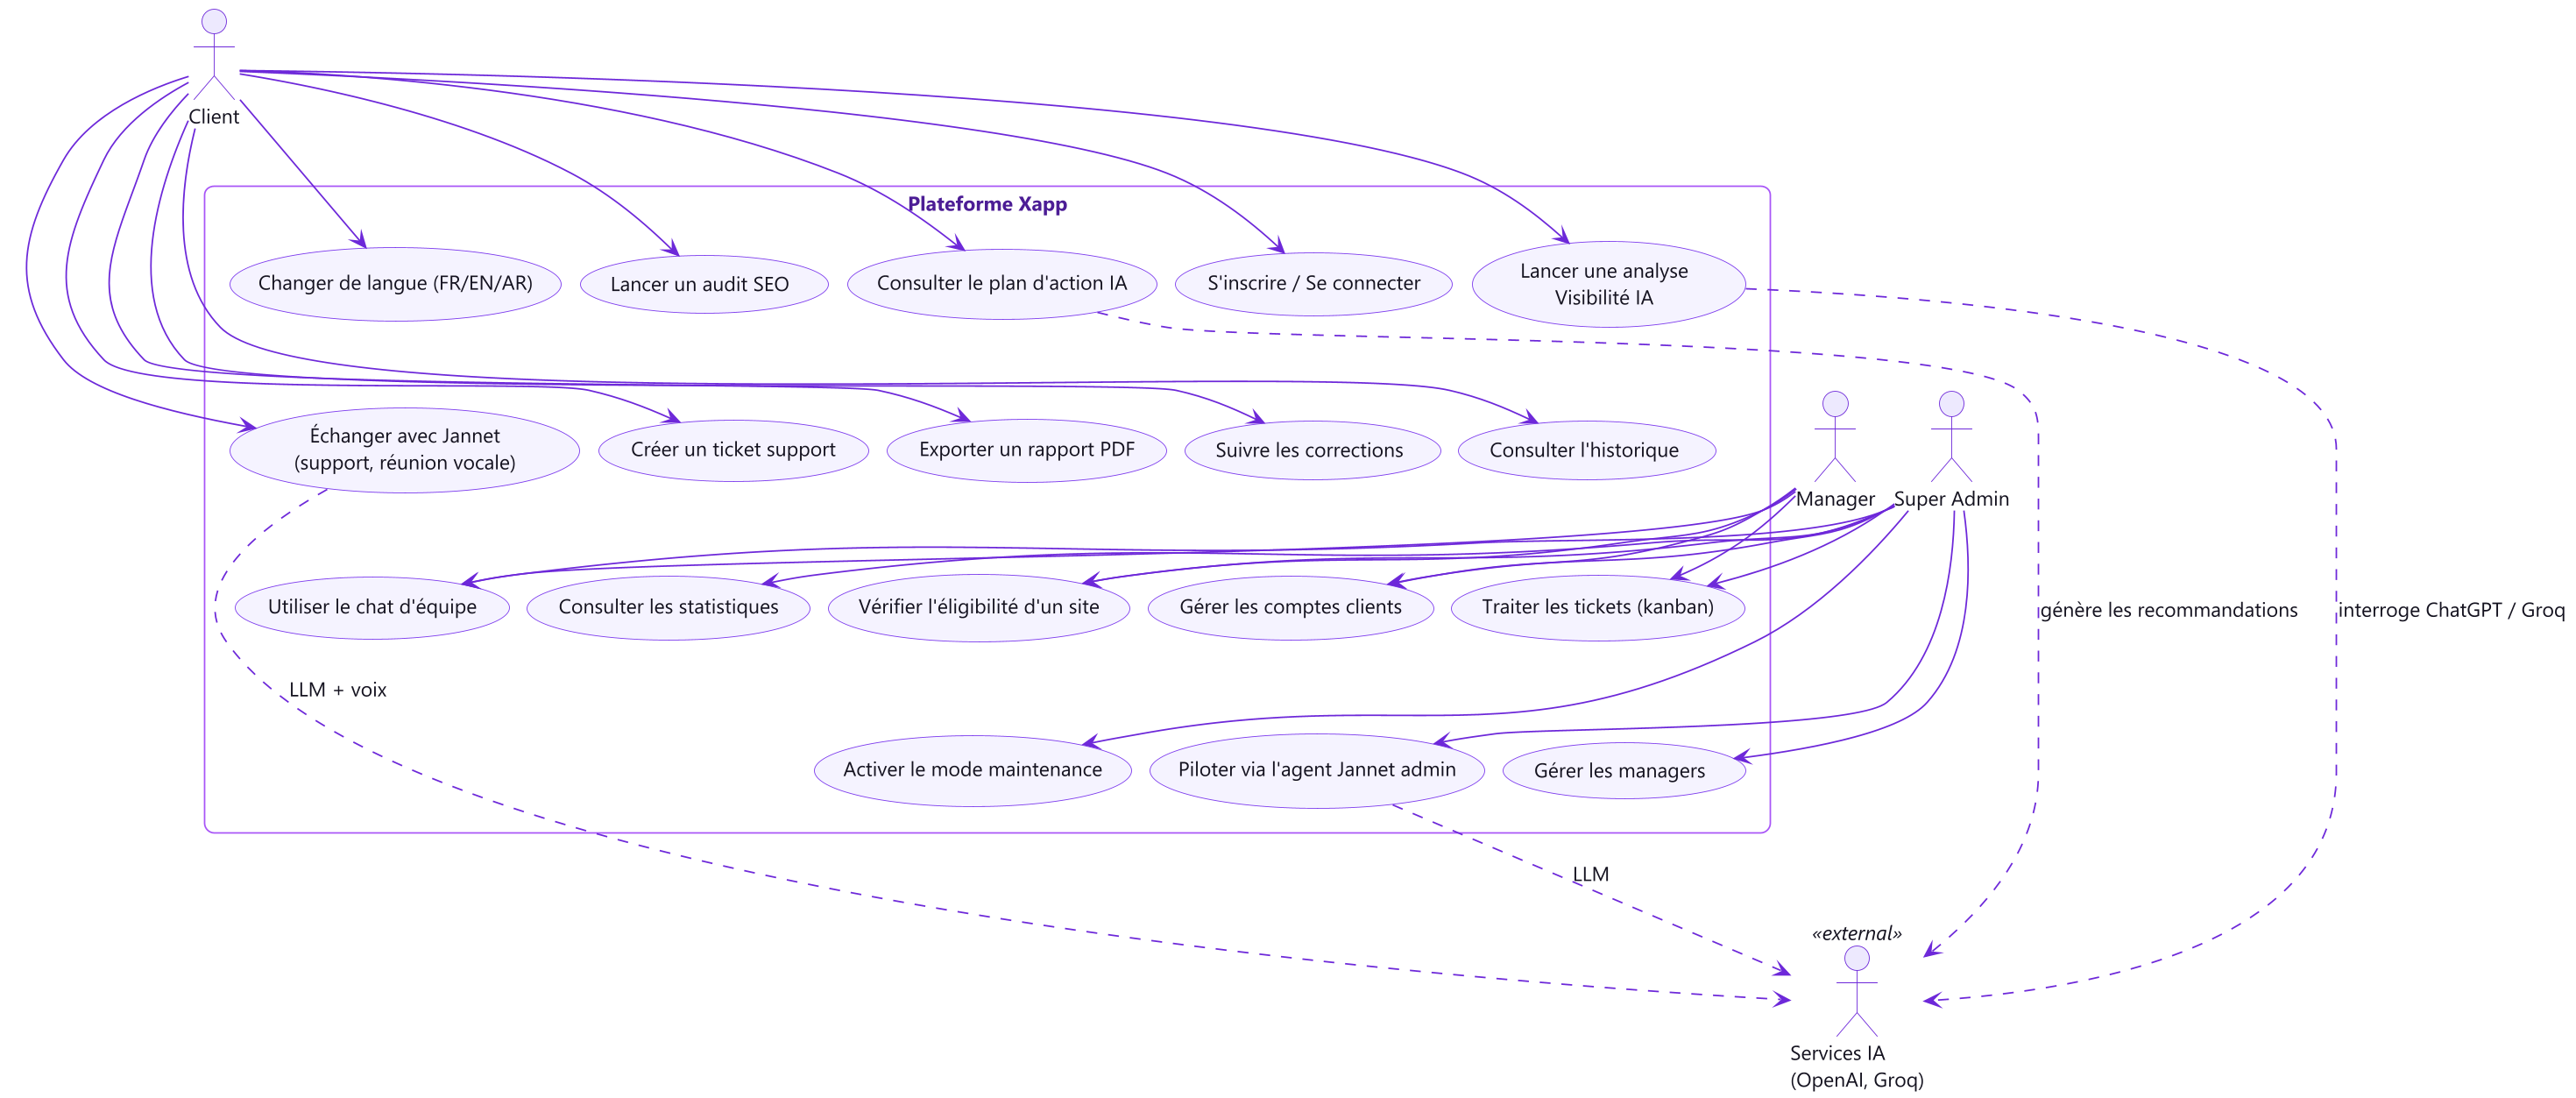
\includegraphics[width=\textwidth,height=0.8\textheight,keepaspectratio]{figures/uml/use_case.png}
  \caption{Diagramme de cas d'utilisation général de la plateforme}\label{fig-cu-global}
\end{figure}

\todo{vérifier que le diagramme de cas d'utilisation reste lisible à l'impression ; sinon le passer sur une page à l'italienne ou le découper par acteur}

\section{Planification par sprint et backlog}
Le backlog du produit a été construit à partir des modules du cahier des charges. Chaque entrée est une histoire utilisateur courte, rattachée à un sprint. Le \cref{tab-backlog} en donne les éléments principaux ; les détails de chaque sprint sont repris dans les chapitres suivants.

\begin{table}[htbp]
\centering
\small
\caption{Backlog du produit (extrait par sprint)}\label{tab-backlog}
\begin{tabularx}{\textwidth}{@{}lXl@{}}
\toprule
\textbf{Sprint} & \textbf{Histoire utilisateur} & \textbf{Priorité}\\
\midrule
\multirow{4}{*}{1} & En tant que visiteur, je veux créer un compte et confirmer mon e-mail & Haute\\
 & En tant qu'utilisateur, je veux me connecter et retrouver mon espace selon mon rôle & Haute\\
 & En tant qu'utilisateur, je veux réinitialiser mon mot de passe par un code reçu par e-mail & Moyenne\\
 & En tant qu'administrateur, je veux créer, modifier et supprimer des comptes & Haute\\
\midrule
\multirow{5}{*}{2} & En tant que client, je veux auditer la page d'accueil de mon site gratuitement & Haute\\
 & En tant que client Pro, je veux auditer tout mon site sans attendre devant l'écran & Haute\\
 & En tant que client, je veux un score sur 100 détaillé par catégorie et par page & Haute\\
 & En tant que client, je veux comparer mon site à mes concurrents & Moyenne\\
 & En tant que client, je veux exporter un rapport PDF & Moyenne\\
\midrule
\multirow{4}{*}{3} & En tant que client, je veux savoir si ChatGPT cite mon site & Haute\\
 & En tant que client, je veux un score AEO/GEO et des recommandations & Haute\\
 & En tant que client, je veux un plan d'action sur deux semaines & Haute\\
 & En tant que client, je veux vérifier qu'une correction est prise en compte & Haute\\
\midrule
\multirow{5}{*}{4} & En tant que client, je veux poser mes questions à un assistant et ouvrir un ticket & Moyenne\\
 & En tant que client, je veux discuter à voix haute de mon audit & Basse\\
 & En tant que manager, je veux traiter les tickets sur un tableau Kanban & Moyenne\\
 & En tant qu'administrateur, je veux confier des actions à un agent IA et pouvoir les annuler & Moyenne\\
 & En tant que client, je veux acheter des crédits en dinars & Haute\\
\bottomrule
\end{tabularx}
\end{table}

\section{Maquettes}
Les maquettes ont porté sur trois écrans clés : la page d'accueil, le tableau de bord et la page d'audit. Une charte graphique commune a été fixée dès le départ : fond sombre pour la navigation, violet comme couleur d'accent (reprise du logo \xapp), cartes arrondies pour le contenu et jauges circulaires pour les scores. \todo{si des maquettes Figma ou papier existent, ajouter ici 2 ou 3 figures (landing, tableau de bord, audit) ; sinon conserver ce paragraphe et le mentionner honnêtement au jury}

\section{Conclusion}
À l'issue du sprint~0, nous disposons d'un périmètre clair : six des sept modules du cahier des charges sont réalisés et le module de monétisation l'est partiellement, auxquels s'ajoute un ensemble d'outils de collaboration. Le chapitre suivant décrit l'architecture technique qui doit les porter.

\chapter{Conception et architecture}

\section{Introduction}
Ce chapitre explique comment le système est construit. Nous justifions d'abord les technologies retenues, puis nous décrivons l'architecture logique, l'architecture physique et le modèle de données. Nous détaillons enfin le scénario dont la logique est la plus fine, l'audit asynchrone d'un site, au moyen de diagrammes de séquence. Les diagrammes UML suivent la notation standard \cite{omguml}.

\section{Choix technologiques}
Le cahier des charges recommandait une API en Python, une interface React et une base relationnelle. Notre pile (\cref{fig-stack}) suit ces recommandations ; le \cref{tab-techno} justifie chaque choix.

\fig[0.9]{figures/architecture/stack_logos.jpeg}{Principales technologies de \xapp}{fig-stack}
\source{schéma réalisé pour la présentation du projet}

\begin{table}[htbp]
\centering
\small
\caption{Technologies retenues et justification}\label{tab-techno}
\begin{tabularx}{\textwidth}{@{}p{2.6cm}p{3.6cm}X@{}}
\toprule
\textbf{Couche} & \textbf{Technologie} & \textbf{Raison du choix}\\
\midrule
Interface & Next.js~16, React~19, TypeScript, Tailwind CSS \cite{nextjsdocs,reactdocs} & Routage par fichiers (App Router), rendu serveur des pages publiques utile au référencement de la plateforme elle-même, typage, écosystème riche (Recharts, Framer Motion)\\
Internationalisation & next-intl & Trois langues (FR, EN, AR) avec bascule \gls{rtl} pour l'arabe, messages centralisés en JSON\\
API & Python, FastAPI, Uvicorn \cite{fastapidocs} & Python est le langage naturel de l'analyse HTML (BeautifulSoup) et des SDK d'IA ; FastAPI est asynchrone, valide les entrées par Pydantic et génère la documentation Swagger \cite{fielding2000rest}\\
Accès aux données & SQLAlchemy \cite{sqlalchemydocs} & \gls{orm} mature ; le même code fonctionne sur SQLite en développement et PostgreSQL en production via \code{DATABASE\_URL}\\
Base de données & PostgreSQL (production), SQLite (développement) \cite{postgresqldocs} & Intégrité référentielle pour les crédits et paiements, colonnes texte pour stocker les résultats d'audit en JSON\\
Crawl et analyse & aiohttp, httpx, BeautifulSoup4, lxml & Requêtes HTTP concurrentes et asynchrones, analyse robuste de HTML imparfait\\
Performance & Google PageSpeed Insights API \cite{pagespeeddocs} & Core Web Vitals mesurés par Google (\gls{lcp}, \gls{cls}, \gls{inp}) plutôt que recalculés\\
Intelligence artificielle & OpenAI (GPT-4o, GPT-4o-mini), Groq \cite{openaidocs,groqdocs} & OpenAI pour le plan d'action et la présence dans ChatGPT ; Groq pour Jannet et la transcription (Whisper), rapide et à faible coût\\
PDF & ReportLab & Génération côté serveur de rapports et plans d'action signés\\
Paiement & Flouci \cite{flouci} & Passerelle tunisienne permettant de payer en dinars\\
Hébergement & VPS Ubuntu, Nginx, systemd, PM2, GitHub Actions \cite{nginxdocs,pm2docs} & Contrôle complet de l'environnement, coût fixe, déploiement automatique à chaque push\\
\bottomrule
\end{tabularx}
\end{table}

\subsection{Pourquoi deux langages ?}
Le choix d'un front en TypeScript et d'une API en Python impose deux écosystèmes. Nous l'avons assumé parce que chaque côté profite de son meilleur outillage : l'analyse de pages, le calcul des scores et les appels aux modèles de langage sont plus simples en Python, tandis que Next.js offre un rendu serveur et une internationalisation que les cadriciels Python n'égalent pas. Le contrat entre les deux est une API REST en JSON, authentifiée par jeton, documentée automatiquement par FastAPI.

\subsection{Pourquoi pas de file de messages ?}
Un audit Pro dure de quelques dizaines de secondes à plusieurs minutes, bien au-delà de la centaine de secondes qu'autorise le proxy Cloudflare placé devant le serveur. La solution classique serait une file de messages (Redis et Celery). Nous avons préféré un exécuteur intégré à FastAPI : une boucle asyncio, lancée au démarrage, qui traite les jobs enregistrés en base un par un. Ce choix évite un service supplémentaire sur un serveur unique ; il limite en contrepartie le débit à un audit lourd à la fois, ce que nous discutons au chapitre~\ref{chap-deploiement}.

\section{Architecture logique}
L'application suit une architecture client-serveur découplée en couches (\cref{fig-archi-logique}).

\begin{figure}[htbp]
\centering
\begin{tikzpicture}[every node/.style={font=\small},
  box/.style={draw,rounded corners,fill=grisclair,minimum width=3.4cm,minimum height=0.9cm,align=center},
  ext/.style={draw,rounded corners,fill=jauneaw!25,minimum width=2.8cm,minimum height=0.8cm,align=center},
  lab/.style={font=\footnotesize,fill=white,inner sep=1pt},
  arr/.style={-{Stealth[length=2mm]},thick}]
  \node[box] (nav) at (0,0) {Navigateur\\(FR / EN / AR)};
  \node[box] (front) at (0,-2) {Frontend Next.js~16\\React~19, next-intl};
  \node[box,minimum width=5.6cm] (api) at (0,-4.4) {API FastAPI\\auth, audit, ai-visibility, admin,\\jannet, tickets, team-chat\ldots};
  \node[box] (engine) at (-2.3,-6.9) {Moteur d'audit\\(crawl, scoring)};
  \node[box] (runner) at (2.3,-6.9) {Exécuteur\\asynchrone};
  \node[box] (db) at (0,-9) {SQLAlchemy\\PostgreSQL / SQLite};
  \node[ext] (google) at (6.6,-3.2) {PageSpeed, GSC};
  \node[ext] (ia) at (6.6,-4.4) {OpenAI, Groq};
  \node[ext] (pay) at (6.6,-5.6) {Flouci, SMTP};
  \draw[arr] (nav)--node[lab,right=2pt]{HTTPS}(front);
  \draw[arr] (front)--node[lab,left=2pt]{REST + JWT, SSE, WebSocket}(api);
  \draw[arr] (api)--(engine); \draw[arr] (api)--(runner);
  \draw[arr] (engine)--(db); \draw[arr] (runner)--(db);
  \draw[arr] (api.east)--(ia.west); \draw[arr] (api.east)--(google.west); \draw[arr] (api.east)--(pay.west);
\end{tikzpicture}
\caption{Architecture logique en couches}\label{fig-archi-logique}
\end{figure}

\paragraph{Couche présentation (Next.js).} L'interface utilise l'App Router : chaque dossier de \route{app/} correspond à une route (\route{/dashboard/analyse}, \route{/dashboard/ai-visibility}, etc.). Les pages publiques (accueil en trois langues, méthodologie du score, pages légales) bénéficient du rendu serveur. Un client Axios unique (\code{lib/api.ts}) ajoute le jeton à chaque requête et redirige vers la connexion en cas d'erreur 401. Un contexte React (\code{SubscriptionContext}) expose en temps réel le plan, les crédits et les fonctionnalités débloquées, ce qui permet d'afficher ou de verrouiller les menus.

\paragraph{Couche applicative (FastAPI).} Elle est organisée en routeurs par domaine : authentification, administration, audits et visibilité IA (dans \code{main.py}), Jannet, réunion vocale, paiements, export PDF, notifications, messagerie d'équipe et tickets. Plus d'une centaine de routes REST sont exposées ; la liste par domaine figure en annexe. Les dépendances FastAPI (\code{get\_current\_user}, \code{get\_admin\_user}) appliquent l'authentification et les rôles. Un service dédié (\code{services/credit\_service.py}) concentre la logique des crédits.

\paragraph{Moteur d'audit.} Le paquet \code{audit/} est une bibliothèque interne indépendante de l'API : crawl, analyse de page, audits vitrine et e-commerce, score du site complet, PageSpeed, visibilité IA et présence dans les réponses des modèles. Il peut être appelé de façon synchrone (audit de la page d'accueil) ou par l'exécuteur asynchrone (audit Pro).

\paragraph{Couche données.} Dix-huit tables décrivent les entités (\cref{sec-modele-donnees}). Les résultats d'audit, volumineux et de structure variable, sont stockés en JSON dans une colonne texte, à côté des colonnes qui servent aux recherches (score, type, date).

\paragraph{Canaux temps réel.} En plus du REST, deux canaux poussent des données vers le navigateur : un flux \gls{sse} pour afficher progressivement les réponses des moteurs IA, et une connexion WebSocket authentifiée pour les notifications.

\section{Architecture physique et déploiement}
En production, tout tourne sur un unique serveur privé virtuel Ubuntu (\cref{fig-deploiement}). Cloudflare assure le DNS ; Nginx reçoit les requêtes en HTTPS (port~443), termine le chiffrement TLS avec un certificat Let's Encrypt et route les chemins \route{/api}, \route{/auth}, \route{/audit} et \route{/admin} vers l'API (Uvicorn, port~8000, supervisé par systemd), et tout le reste vers le serveur Next.js (port~3000, supervisé par PM2). PostgreSQL tourne sur la même machine et n'est pas exposé à Internet. \todo{indiquer les caractéristiques du VPS (processeur, mémoire, disque), la version d'Ubuntu et de PostgreSQL}

\fig[0.95]{figures/architecture/deploiement.png}{Diagramme de déploiement}{fig-deploiement}
\source{diagramme PlantUML du dépôt (\code{docs/uml/deployment.puml})}

\section{Modèle de données}\label{sec-modele-donnees}
Le diagramme de classes de la \cref{fig-classes} présente les entités principales. Il est présenté sur une page à l'italienne pour rester lisible.

\begin{landscape}
\begin{figure}[p]
  \centering
  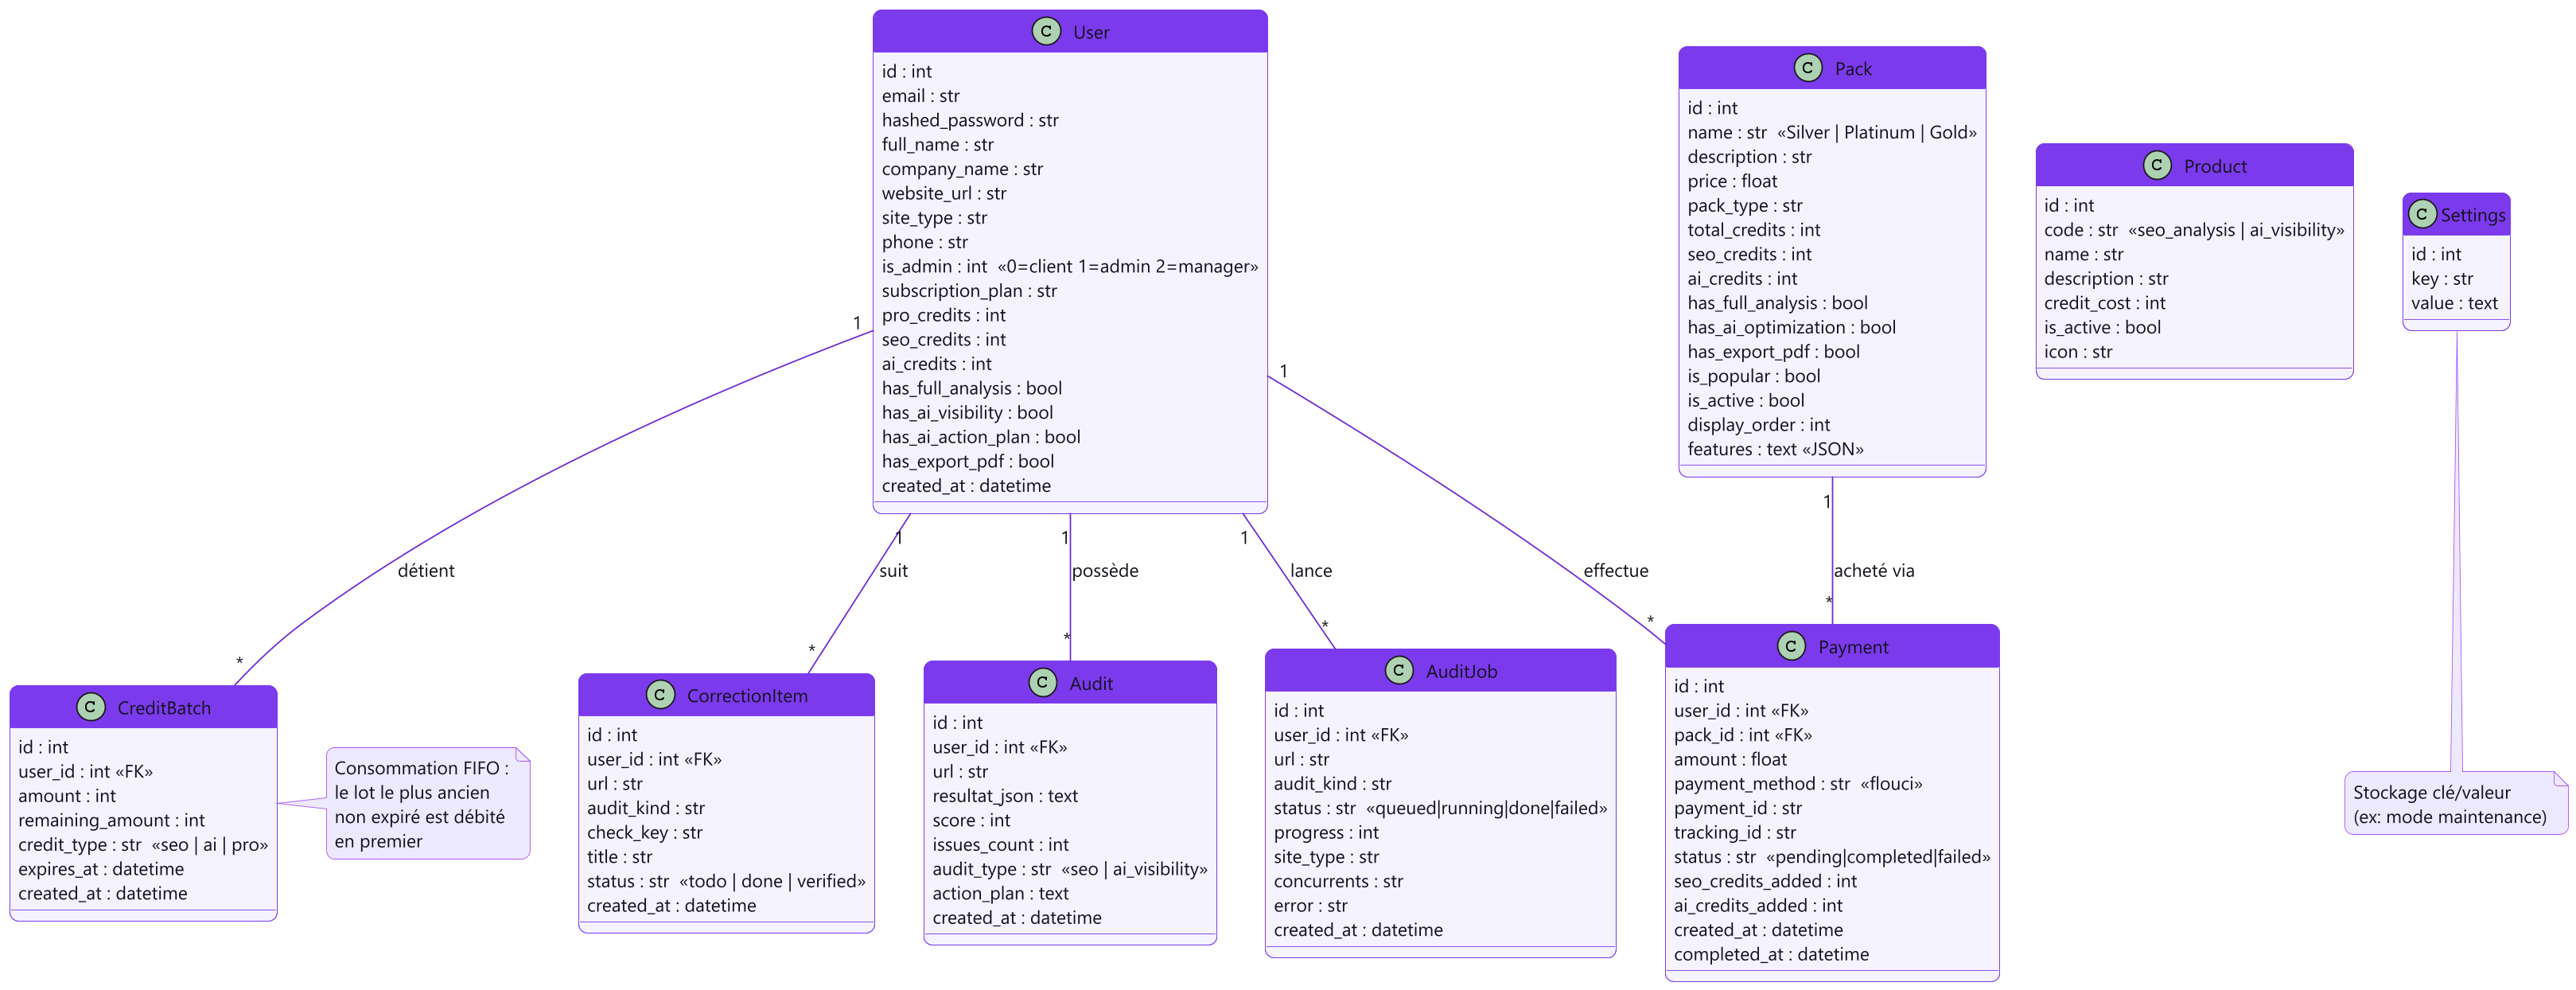
\includegraphics[width=0.96\linewidth,height=0.8\textheight,keepaspectratio]{figures/uml/class_diagram.png}
  \caption{Diagramme de classes (modèles SQLAlchemy principaux)}\label{fig-classes}
\end{figure}
\end{landscape}

\todo{le diagramme de classes ne montre que 9 entités sur 18 ; ajouter les tables de collaboration (tickets, messages, notifications, chat, agent, exports) ou préciser dans la légende qu'il s'agit du cœur métier}

Le \cref{tab-collections} donne le rôle de chaque table.

\begin{table}[htbp]
\centering
\small
\caption{Tables de la base de données et rôle}\label{tab-collections}
\begin{tabularx}{\textwidth}{@{}p{4.2cm}X@{}}
\toprule
\textbf{Table} & \textbf{Rôle}\\
\midrule
\code{users} & Compte, rôle (\code{is\_admin}), plan, soldes de crédits, fonctionnalités débloquées, codes de vérification et de réinitialisation, jeton Search Console\\
\code{audits} & Résultat d'un audit SEO ou IA (JSON), score, nombre de problèmes, plan d'action enregistré\\
\code{audit\_jobs} & Job asynchrone : statut, progression, pages analysées, tranche de pages, crédit utilisé et remboursement\\
\code{correction\_items} & Correction à effectuer : catégorie, gravité, pages concernées, statut, historique\\
\code{credit\_batches} & Lot de crédits avec type, montant restant et date d'expiration\\
\code{packs}, \code{products} & Offres commerciales et coût en crédits de chaque action\\
\code{payments} & Paiements (Flouci), statut, crédits ajoutés\\
\code{exports} & Rapports PDF générés avec leur signature\\
\code{tickets}, \code{ticket\_messages} & Tickets de support et leurs échanges\\
\code{knowledge\_entries} & Base de connaissances de Jannet, alimentée par les tickets résolus\\
\code{agent\_actions} & Journal des actions de l'agent Jannet, avec données d'annulation\\
\code{notifications} & Notifications persistées\\
\code{chat\_channels}, \code{chat\_channel\_members}, \code{chat\_messages} & Messagerie d'équipe : canal général et conversations privées\\
\code{settings} & Paramètres clé/valeur (mode maintenance)\\
\bottomrule
\end{tabularx}
\end{table}

Quelques décisions de modélisation méritent d'être signalées.

\begin{itemize}
  \item \textbf{Crédits en lots.} Le solde affiché sur l'utilisateur n'est qu'un cache ; la vérité est dans \code{credit\_batches}. Chaque achat crée un lot daté, avec une expiration, et la consommation débite d'abord le lot non expiré le plus ancien (\gls{fifo}).
  \item \textbf{Résultats en JSON.} La structure d'un résultat d'audit change selon le type (vitrine, e-commerce, IA) et a évolué au fil des sprints. La stocker en JSON évite une migration à chaque nouvel indicateur.
  \item \textbf{Job distinct de l'audit.} \code{audit\_jobs} décrit l'exécution (file, progression, erreur), \code{audits} le résultat. Un job échoué n'encombre pas l'historique et son crédit peut être remboursé.
  \item \textbf{Corrections identifiées par clé.} Chaque correction porte une clé machine (\code{check\_key}) qui permet à la fois d'éviter les doublons d'un audit à l'autre et de revérifier précisément ce point.
\end{itemize}

\section{Diagrammes de séquence}

\subsection{Audit SEO asynchrone}
Le scénario se découpe en deux phases : le lancement (\cref{fig-seq-audit-1}) et le traitement en arrière-plan avec le suivi de progression (\cref{fig-seq-audit-2}).

\fig[0.95]{figures/uml/sequence_audit_1.png}{Séquence : lancement d'un audit et consommation du crédit}{fig-seq-audit-1}

Au lancement, le client saisit l'adresse de son site. L'API vérifie le jeton, débite un crédit selon la règle FIFO, crée un job à l'état \code{queued} et répond immédiatement avec son identifiant (code~202). L'utilisateur n'attend donc pas la fin du crawl pour récupérer la main.

\fig[0.95]{figures/uml/sequence_audit_2.png}{Séquence : traitement en arrière-plan et suivi de progression}{fig-seq-audit-2}

L'exécuteur récupère le job, le passe à \code{running}, lance le crawl et l'analyse des pages, met à jour la progression en base et enregistre le résultat. Pendant ce temps, le frontend interroge \route{/audit/status/\{job\_id\}} toutes les trois secondes. En cas d'échec ou de dépassement du budget de 600~secondes, le job passe à \code{failed} et le crédit est remboursé.

\section{Conclusion}
L'architecture retenue sépare nettement l'interface, l'API, le moteur d'audit et les données, et isole les traitements longs dans un exécuteur asynchrone. Le chapitre suivant aborde la réalisation, en commençant par le socle commun à tous les modules : les comptes et le contrôle d'accès.

\chapter{Sprint 1 : socle, comptes et contrôle d'accès}

\section{Introduction}
Tout le reste de la plateforme dépend de la réponse à une question simple : qui est cette personne et que peut-elle faire ? Le premier sprint a donc posé les bases communes : inscription, vérification de l'adresse e-mail, connexion, réinitialisation de mot de passe, rôles et premières pages d'administration. Nous y avons aussi installé le socle technique (structure du projet, déploiement continu) pour pouvoir livrer dès la suite.

\section{Backlog du sprint}
\begin{table}[htbp]
\centering
\small
\caption{Backlog du sprint 1}\label{tab-backlog-s1}
\begin{tabularx}{\textwidth}{@{}lXl@{}}
\toprule
\textbf{Réf.} & \textbf{Tâche} & \textbf{État}\\
\midrule
S1.1 & Mise en place du projet FastAPI et du projet Next.js, configuration SQLite/PostgreSQL & Terminé\\
S1.2 & Déploiement continu sur le VPS par GitHub Actions (Nginx, systemd, PM2) & Terminé\\
S1.3 & Inscription publique avec reCAPTCHA & Terminé\\
S1.4 & Vérification d'adresse e-mail par code à six chiffres & Terminé\\
S1.5 & Connexion, émission et vérification d'un jeton JWT & Terminé\\
S1.6 & Réinitialisation de mot de passe par code OTP envoyé par e-mail & Terminé\\
S1.7 & Rôles client, manager et super admin ; dépendances de contrôle côté API & Terminé\\
S1.8 & Console d'administration : liste, création, modification, suppression des comptes & Terminé\\
S1.9 & Profil : nom, entreprise, site, téléphone, photo, mot de passe & Terminé\\
S1.10 & Page d'accueil, tableau de bord et pages légales & Terminé\\
\bottomrule
\end{tabularx}
\end{table}

\section{Conception de l'authentification}

\subsection{Principes retenus}
Nous avons choisi une authentification à base de jetons \gls{jwt} \cite{rfc7519}. À la connexion, le serveur vérifie le mot de passe, puis signe (algorithme HS256) un jeton contenant l'adresse de l'utilisateur, valable vingt-quatre heures. Le client le conserve et l'envoie dans l'en-tête \code{Authorization} de chaque requête. Ce modèle sans état évite de stocker des sessions côté serveur.

Le jeton ne contient pas le rôle : à chaque requête protégée, la dépendance \code{get\_current\_user} décode le jeton puis relit l'utilisateur en base. Si un administrateur modifie un rôle, retire des droits ou supprime un compte, l'effet est immédiat.

\subsection{Stockage des mots de passe}
Les mots de passe sont hachés avec bcrypt \cite{provos1999bcrypt} via la bibliothèque passlib. Le serveur n'enregistre jamais le mot de passe en clair. \todo{indiquer la longueur minimale de mot de passe effectivement imposée côté client et côté serveur}

\subsection{Inscription et vérification d'adresse}
Le parcours d'inscription comporte plusieurs garde-fous (\cref{fig-seq-inscription}) :
\begin{enumerate}
  \item le formulaire est protégé par Google reCAPTCHA, pour limiter les inscriptions automatisées ;
  \item le serveur refuse une adresse déjà utilisée, crée le compte en plan \code{free} et à l'état « non vérifié » ;
  \item un code à six chiffres, valable vingt-quatre heures, est envoyé par e-mail ; l'utilisateur le saisit sur la page \route{/verify-email} et peut en demander un nouveau.
\end{enumerate}

\begin{figure}[htbp]
\centering
\begin{tikzpicture}[node distance=7mm and 10mm, every node/.style={font=\small}, box/.style={draw,rounded corners,fill=grisclair,minimum width=2.6cm,minimum height=0.8cm,align=center}, arr/.style={-{Stealth[length=2mm]},thick}]
  \node[box] (a) {Formulaire\\+ reCAPTCHA};
  \node[box,right=of a] (b) {Création du\\compte (free)};
  \node[box,right=of b] (c) {Envoi du\\code (24\,h)};
  \node[box,right=of c] (d) {Saisie du\\code};
  \node[box,below=of d,fill=jauneaw!30] (e) {Compte\\vérifié};
  \node[box,below=of b,fill=rougeatodo!15] (f) {Adresse déjà\\utilisée : refus};
  \draw[arr] (a)--(b); \draw[arr] (b)--(c); \draw[arr] (c)--(d); \draw[arr] (d)--(e);
  \draw[arr,dashed] (a)|-(f);
\end{tikzpicture}
\caption{Parcours d'inscription et de vérification}\label{fig-seq-inscription}
\end{figure}

\todo{préciser si la connexion est refusée tant que l'adresse n'est pas vérifiée, ou si seules certaines fonctions sont bloquées}

\subsection{Mot de passe oublié}
La réinitialisation se fait en trois étapes : la demande (\route{/auth/forgot-password}) envoie un code \gls{otp} à six chiffres valable une heure ; la vérification du code (\route{/auth/verify-reset-code}) renvoie un jeton de réinitialisation à durée limitée ; ce jeton permet enfin de choisir un nouveau mot de passe (\route{/auth/reset-password}). Le code saisi n'est donc jamais réutilisable pour une autre opération. \todo{vérifier que la demande répond par le même message que l'adresse existe ou non (anti-énumération)}

\figmanquante{fig-login}{Page de connexion}{Capturer la page /login (version française et, si possible, version arabe en RTL), avec le formulaire e-mail et mot de passe et le lien « Mot de passe oublié ».}

\figmanquante{fig-inscription}{Page d'inscription et saisie du code de vérification}{Capturer /register avec le reCAPTCHA visible, puis /verify-email où l'on saisit le code à six chiffres.}

\section{Contrôle d'accès par rôles}
Le contrôle d'accès (\gls{rbac}) se fait à deux niveaux qui se complètent.

\paragraph{Côté interface.} Le tableau de bord vérifie la présence du jeton et charge le profil ; la barre latérale (\code{Sidebar.tsx}) affiche ou verrouille les menus selon le plan et les fonctionnalités débloquées. L'administration est servie sous des chemins distincts du tableau de bord client, avec leur propre page de connexion. Ces contrôles améliorent l'ergonomie mais ne constituent pas une barrière de sécurité.

\paragraph{Côté serveur.} C'est ici que se joue la sécurité réelle. Les routes clientes dépendent de \code{get\_current\_user} ; les routes d'administration de \code{get\_admin\_user}, qui exige \code{is\_admin} supérieur ou égal à~1. Les opérations critiques (suppression de compte, maintenance, actions mutantes de l'agent Jannet) sont réservées au super admin (\code{is\_admin = 1}). Les fonctionnalités payantes sont vérifiées au moment de l'appel : un client sans le drapeau \code{has\_ai\_visibility} ou sans crédit reçoit un refus explicite.

\begin{table}[htbp]
\centering
\small
\caption{Accès par espace et par rôle}\label{tab-acces-roles}
\setlength{\tabcolsep}{4pt}
\begin{tabular}{@{}p{4.6cm}p{4.2cm}cccc@{}}
\toprule
\textbf{Espace} & \textbf{Chemin} & \rotatebox{60}{\textbf{Free}} & \rotatebox{60}{\textbf{Pro}} & \rotatebox{60}{\textbf{Manager}} & \rotatebox{60}{\textbf{Super admin}}\\
\midrule
Public & \route{/}, \route{/en}, \route{/ar}, \route{/methodologie-score} & \ding{51} & \ding{51} & \ding{51} & \ding{51}\\
Tableau de bord, audit de la page d'accueil, historique & \route{/dashboard}, \route{/dashboard/analyse} & \ding{51} & \ding{51} & --- & ---\\
Audit Pro, visibilité IA, plan d'action, corrections, comparateur & \route{/dashboard/ai-visibility}, \ldots & --- & \ding{51} & --- & ---\\
Gestion des clients et des crédits & \route{/ingbxweb/clients} & --- & --- & \ding{51} & \ding{51}\\
Packs, maintenance, journaux, actions Jannet & chemin d'administration réservé & --- & --- & --- & \ding{51}\\
Tickets Kanban, messagerie d'équipe & administration & --- & --- & \ding{51} & \ding{51}\\
\bottomrule
\end{tabular}
\end{table}
\todo{vérifier chaque case du tableau en testant avec un compte de chaque rôle ; ne pas publier le chemin exact de la console super admin}

\section{Gestion des comptes par l'administrateur}
La console d'administration propose la liste des comptes avec recherche, la création d'un compte, la modification du profil, du rôle et du plan, la suppression, ainsi que l'ajout ou la définition exacte des crédits. Une route de statistiques agrège le nombre de comptes, de clients Pro et d'audits ; elle alimente le tableau de bord administrateur. Une fonction de données de démonstration permet de préparer un compte complet pour une présentation commerciale.

\fig[0.95]{figures/captures/utilisateurs.png}{Console d'administration : liste des utilisateurs}{fig-admin-console}
\source{capture d'écran de l'application}

\section{Profil et tableau de bord}
Le client complète son profil (nom, entreprise, site, type de site, téléphone, photo). Le site renseigné pré-remplit les formulaires d'audit. Le tableau de bord (\cref{fig-dashboard}) résume les derniers scores, le solde de crédits et les raccourcis vers les modules.

\fig[0.95]{figures/captures/dashboard.png}{Tableau de bord du client}{fig-dashboard}
\source{capture d'écran de l'application}

\section{Courriels transactionnels}
Les courriels (code de vérification, code de réinitialisation, confirmation de ticket, notifications) sont envoyés par SMTP via un relais Brevo, avec une mise en page aux couleurs de \xapp. Une route d'administration permet d'envoyer un courriel de test pour diagnostiquer la configuration.

\section{Bilan du sprint}
\subsection{Livrables}
Les comptes, l'authentification, les rôles et l'administration des utilisateurs sont en production, ainsi que la chaîne de déploiement continu. Les parcours critiques ont été testés manuellement. \todo{confirmer}

\subsection{Rétrospective}
\begin{description}[leftmargin=1.2em,style=nextline]
  \item[Ce qui a bien fonctionné.] Mettre en place le déploiement continu dès le premier sprint a permis de tester chaque fonctionnalité dans les conditions réelles (HTTPS, Cloudflare, nom de domaine).
  \item[Ce qui a posé problème.] La clé reCAPTCHA, liée au domaine, a dû être régénérée lors du passage au domaine définitif ; elle a temporairement bloqué la connexion de l'administrateur, et la vérification a été rendue facultative à la connexion. \todo{confirmer ce récit à partir de l'historique Git et de votre souvenir}
  \item[À améliorer.] Le jeton est conservé dans le stockage local du navigateur, ce qui l'expose en cas de faille XSS ; un cookie \code{HttpOnly} serait plus sûr. Les codes de vérification sont stockés en clair ; les stocker sous forme de condensat réduirait l'impact d'une fuite de la base.
\end{description}

\section{Conclusion}
Ce sprint a livré le socle du système : identité, rôles, sécurité d'accès et déploiement. Le sprint suivant s'appuie dessus pour construire le cœur de la valeur : le moteur d'audit SEO.

\chapter{Sprint 2 : moteur d'audit SEO}

\section{Introduction}
Ce sprint construit le cœur de \xapp{} : le moteur qui parcourt un site, analyse chaque page et calcule un score. C'est aussi le sprint qui a rencontré les contraintes les plus concrètes : des sites lents, des sites immenses, des protections anti-robots, et un proxy qui coupe toute requête au-delà d'une centaine de secondes.

\section{Backlog du sprint}
\begin{table}[htbp]
\centering
\small
\caption{Backlog du sprint 2}\label{tab-backlog-s2}
\begin{tabularx}{\textwidth}{@{}lXl@{}}
\toprule
\textbf{Réf.} & \textbf{Tâche} & \textbf{État}\\
\midrule
S2.1 & Analyse unitaire d'une page (titre, méta-description, Hn, images, liens, canonical, robots) & Terminé\\
S2.2 & Audit gratuit de la page d'accueil (vitrine basique) & Terminé\\
S2.3 & Détection et analyse de \code{robots.txt} et du sitemap XML & Terminé\\
S2.4 & Crawl multi-pages concurrent et audit Pro & Terminé\\
S2.5 & Système de scoring sur 100 par catégorie & Terminé\\
S2.6 & Exécuteur asynchrone de jobs, progression, remboursement & Terminé\\
S2.7 & Audit e-commerce (fiches produits, catégories, plateforme) & Terminé\\
S2.8 & Intégration PageSpeed Insights et Google Search Console & Terminé\\
S2.9 & Historique, comparateur de concurrents, suggestion de mots-clés & Terminé\\
S2.10 & Export PDF signé des rapports & Terminé\\
\bottomrule
\end{tabularx}
\end{table}

\section{Analyse d'une page}
L'unité de base du moteur est l'analyse d'une URL. La page est téléchargée de façon asynchrone (aiohttp), puis analysée avec BeautifulSoup. Le \cref{tab-controles} résume les contrôles effectués, regroupés en catégories.

\begin{table}[htbp]
\centering
\small
\caption{Contrôles effectués par le moteur d'audit}\label{tab-controles}
\begin{tabularx}{\textwidth}{@{}p{2.6cm}X@{}}
\toprule
\textbf{Catégorie} & \textbf{Contrôles}\\
\midrule
Technique & HTTPS, code de statut HTTP, temps de réponse, taille du HTML, balise canonical, directives \code{noindex}/\code{nofollow}, balise viewport, liens cassés, \code{robots.txt}, sitemap\\
Contenu & Présence et longueur du titre et de la méta-description, doublons de titres et de méta-descriptions entre pages, nombre de mots, attributs ALT des images\\
Structure & Présence d'un H1 unique, hiérarchie des titres H1--H6, données structurées Schema.org\\
Performance & Temps de chargement mesuré, Core Web Vitals (\gls{lcp}, \gls{cls}, \gls{inp}) et \gls{ttfb} via PageSpeed Insights\\
E-commerce & Type de page (produit, catégorie), schéma \code{Product} (prix, devise, disponibilité, SKU, marque, avis), fil d'Ariane, plateforme détectée (WooCommerce, Shopify\ldots)\\
\bottomrule
\end{tabularx}
\end{table}

Pour ne pas surcharger le site audité, la vérification des liens cassés est limitée à vingt liens par page, par des requêtes \code{HEAD} à concurrence bornée.

\section{Crawl d'un site}
L'audit Pro commence par lire \code{robots.txt} et le sitemap XML (jusqu'à 10\,000 URL, sitemaps imbriqués compris), qui servent à la fois d'indicateurs de qualité et de source d'URL. Le crawl part ensuite de la page d'accueil, suit les liens internes et filtre ce qui n'est pas une page (fichiers, paramètres de pagination, pages non publiées). Une empreinte du contenu permet d'écarter les pages en double. Les requêtes sont envoyées par un nombre limité de travailleurs (trois) avec un délai initial de vingt secondes, pour rester bien en deçà de la limite de Cloudflare.

Le nombre de pages analysées en détail dépend du plan : la page d'accueil seule pour le plan Free, et des tranches de cent pages par crédit pour un audit Pro. En parallèle, un module de « score du site complet » (\code{full\_site.py}) parcourt jusqu'à 5\,000 pages avec une analyse plus légère, pour compter les problèmes à l'échelle du site entier. \todo{confirmer la limite de pages réellement appliquée par plan (40, 100 ou par tranche) et la mettre en cohérence avec la présentation}

\section{Calcul du score}
Le score a été conçu pour être exigeant : un score supérieur à 90 doit être difficile à obtenir, afin que l'outil ne flatte pas l'utilisateur. Le score technique pèse 60~\% du score d'une page ; il combine des notes partielles avec des seuils explicites (\cref{tab-seuils}). Le score de contenu complète les 40~\% restants. Les signaux de niveau site (HTTPS, qualité de \code{robots.txt} et du sitemap) sont intégrés au score technique de chaque page, et les titres ou descriptions dupliqués sont pénalisés.

\begin{table}[htbp]
\centering
\small
\caption{Exemple de barème : temps de chargement d'une page}\label{tab-seuils}
\begin{tabular}{@{}lc@{}}
\toprule
\textbf{Temps de chargement} & \textbf{Note partielle}\\
\midrule
$\leq 700$~ms & 100\\
$\leq 1\,500$~ms & 80\\
$\leq 2\,500$~ms & 60\\
$\leq 4\,000$~ms & 30\\
au-delà & 10\\
\bottomrule
\end{tabular}
\end{table}

Le score du site complet suit une autre logique, fondée sur les problèmes : chaque type de problème a une gravité, et le score vaut
\[ S = 100 \times \left(1 - \frac{\sum_k \frac{n_k}{N}\, g_k}{\sum_k g_k}\right) \]
où $n_k$ est le nombre de pages présentant le problème $k$, $N$ le nombre de pages analysées et $g_k$ la gravité du problème. Une page publique (\route{/methodologie-score}) explique cette méthode aux utilisateurs. \todo{vérifier la répartition exacte 60/40 et la formule finale dans scoring.py et full\_site.py avant la soutenance}

\fig[0.95]{figures/captures/seo_complet.png}{Résultat d'un audit SEO : score global, scores par catégorie et pages analysées}{fig-seo-resultat}
\source{capture d'écran de l'application}

\fig[0.95]{figures/captures/seo_indicateurs.png}{Indicateurs clés d'un audit}{fig-seo-indicateurs}
\source{capture d'écran de l'application}

\section{Exécution asynchrone}
Un audit Pro ne peut pas tenir dans une requête HTTP. Nous l'avons donc confié à un exécuteur intégré (\code{audit\_runner.py}) :
\begin{enumerate}
  \item la route \route{/audit/start} débite le crédit, crée un job \code{queued} et répond aussitôt (code~202) ;
  \item une boucle asyncio, démarrée avec FastAPI, prend les jobs un par un (concurrence~1, pour protéger le serveur), les passe à \code{running} et exécute l'audit vitrine ou e-commerce ;
  \item le moteur met à jour la progression (pourcentage, pages analysées sur pages totales) au fil du crawl ;
  \item à la fin, le résultat est enregistré dans \code{audits}, les corrections sont dérivées (chapitre~\ref{chap-visibilite}) et le job passe à \code{done} ;
  \item en cas d'erreur ou au-delà de 600~secondes, le job passe à \code{failed} et le crédit est remboursé, une seule fois grâce au drapeau \code{credit\_refunded}.
\end{enumerate}

Côté interface, la page d'analyse interroge \route{/audit/status/\{job\_id\}} toutes les trois secondes et affiche une barre de progression.

\begin{lstlisting}[language=Python,caption={Paramètres de l'exécuteur d'audit (extrait)},label={lst-runner}]
# Budget temps large pour un job de fond (le HTTP ne nous limite plus).
JOB_MAX_SECONDS = 600
# Pages détaillées par crédit / par lot.
JOB_PAGES_PER_BATCH = 100
\end{lstlisting}

\section{Intégrations Google}
\paragraph{PageSpeed Insights.} L'API PageSpeed Insights (version~5) fournit, pour la stratégie mobile, les métriques de laboratoire et, quand elles existent, les données terrain (CrUX). Nous les reprenons telles quelles plutôt que de recalculer une performance moins fiable.

\paragraph{Google Search Console.} Le client peut connecter son compte Search Console par \gls{oauth}~2.0, avec la portée en lecture seule \code{webmasters.readonly}. La plateforme conserve le jeton de rafraîchissement, choisit la propriété correspondant au site du client et utilise l'API d'inspection d'URL pour connaître l'état réel d'indexation des pages (cinq inspections en parallèle au plus). \todo{ajouter une capture de la connexion GSC ou de l'état d'indexation, si la fonctionnalité est active en production}

\section{Historique, comparateur et mots-clés}
Chaque audit est conservé et consultable depuis l'historique. Le comparateur met en regard le score du site avec celui de concurrents saisis par l'utilisateur. Une route de suggestion de mots-clés s'appuie sur le contenu de la page et un modèle de langage pour proposer des mots-clés à cibler, que l'utilisateur sélectionne dans une fenêtre dédiée. \todo{préciser le nombre maximal de concurrents réellement accepté (la documentation indique 3)}

\figmanquante{fig-comparateur}{Comparateur de concurrents}{Capturer /dashboard/comparateur avec le site et deux ou trois concurrents comparés.}

\section{Export PDF signé}
Le rapport d'audit et le plan d'action peuvent être exportés en PDF. Le document est produit côté serveur avec ReportLab, aux couleurs de \xapp{} : logo, score, recommandations, puis un pied de page portant une signature calculée par SHA-256 sur l'URL, le score, le type, la date et l'adresse du client. Chaque export est enregistré dans la table \code{exports}. Il s'agit d'une empreinte d'intégrité et non d'une signature électronique au sens juridique. \todo{reformuler la mention « certifié par signature électronique » imprimée sur les PDF, qui peut prêter à confusion}

\section{Bilan du sprint}
\subsection{Livrables}
Le moteur d'audit (page d'accueil, Pro, e-commerce), le scoring, l'exécuteur asynchrone, les intégrations Google, l'historique, le comparateur et l'export PDF sont en production.

\subsection{Rétrospective}
\begin{description}[leftmargin=1.2em,style=nextline]
  \item[Ce qui a bien fonctionné.] Séparer le job de son résultat a rendu le remboursement simple et fiable, et a permis d'afficher une progression réelle.
  \item[Ce qui a posé problème.] Les premières versions exécutaient l'audit dans la requête HTTP ; sur les sites lents ou volumineux, Cloudflare coupait la connexion (erreurs 522 et 524). Il a fallu réduire les délais, borner le crawl, ajouter une route de santé et un outil d'éligibilité, puis passer à l'exécution asynchrone.
  \item[À améliorer.] La concurrence de un job à la fois crée une file d'attente si plusieurs clients lancent un audit simultanément. Les seuils du score ont été fixés empiriquement et mériteraient d'être calibrés sur un échantillon de sites.
\end{description}

\section{Conclusion}
Ce sprint a livré un audit SEO automatique, exigeant et robuste aux sites difficiles. Le sprint suivant ajoute la dimension qui distingue \xapp{} des outils existants : la visibilité dans les moteurs génératifs et la transformation de l'audit en actions.

\chapter{Sprint 3 : visibilité IA, plan d'action et corrections}\label{chap-visibilite}

\section{Introduction}
Ce sprint répond à la deuxième moitié de la problématique : mesurer la visibilité d'un site dans les moteurs génératifs, puis transformer l'ensemble des diagnostics en actions concrètes. Il comprend trois volets : les scores \gls{aeo} et \gls{geo}, le test de présence dans les réponses des modèles de langage, et la chaîne « plan d'action, corrections, vérification ».

\section{Backlog du sprint}
\begin{table}[htbp]
\centering
\small
\caption{Backlog du sprint 3}\label{tab-backlog-s3}
\begin{tabularx}{\textwidth}{@{}lXl@{}}
\toprule
\textbf{Réf.} & \textbf{Tâche} & \textbf{État}\\
\midrule
S3.1 & Score AEO : FAQ, schéma FAQPage, structure des titres, lisibilité, HowTo & Terminé\\
S3.2 & Score GEO : signaux E-E-A-T, schéma Article, cohérence thématique, blocs adaptés à l'IA & Terminé\\
S3.3 & Détection des robots d'IA bloqués et des technologies du site & Terminé\\
S3.4 & Test de présence dans ChatGPT et Groq, analyse des citations & Terminé\\
S3.5 & Diffusion des résultats en flux (SSE) & Terminé\\
S3.6 & Recommandations IA et comparaison avec les concurrents & Terminé\\
S3.7 & Plan d'action généré par IA et export & Terminé\\
S3.8 & Optimisation de contenu (titres, méta-descriptions, textes) & Terminé\\
S3.9 & Checklist de corrections et vérification automatique & Terminé\\
\bottomrule
\end{tabularx}
\end{table}

\section{Des moteurs de recherche aux moteurs génératifs}
Un moteur de recherche classique renvoie une liste de liens ; un moteur génératif rédige une réponse et n'en cite que quelques sources \cite{aggarwal2024geo}. Deux disciplines émergent pour s'y adapter :
\begin{description}[leftmargin=1.2em,style=nextline]
  \item[AEO (\textit{Answer Engine Optimization}).] Structurer le contenu pour qu'il réponde directement à une question : FAQ, blocs question-réponse, données structurées \code{FAQPage} et \code{HowTo} \cite{schemaorg}.
  \item[GEO (\textit{Generative Engine Optimization}).] Rendre le contenu crédible et réutilisable par un modèle : signaux d'expérience, d'expertise, d'autorité et de fiabilité (\gls{eeat}) \cite{googleeeat}, cohérence thématique, citations, statistiques, sémantique HTML.
\end{description}

\section{Scores AEO et GEO}
Chaque score est une somme de composantes plafonnée à 100 (\cref{tab-aeo-geo}). Le score de préparation IA est la moyenne des deux.

\begin{table}[htbp]
\centering
\small
\caption{Composantes des scores AEO et GEO}\label{tab-aeo-geo}
\begin{tabularx}{\textwidth}{@{}p{1.4cm}X@{}}
\toprule
\textbf{Score} & \textbf{Composantes}\\
\midrule
AEO & Présence d'une FAQ et nombre de questions, schéma \code{FAQPage}, hiérarchie des titres valide, lisibilité du texte (25~\% du score de lisibilité), schéma \code{HowTo}, blocs de réponse courts\\
GEO & Signaux E-E-A-T (35~\% : auteur, dates, mentions légales, contact, références), schéma \code{Article} (15 points), cohérence thématique (jusqu'à 15 points), blocs adaptés à l'IA (listes, tableaux, définitions), performance (10~\%), sémantique HTML (10~\%)\\
Global & $\text{score IA} = 0{,}5 \times \text{AEO} + 0{,}5 \times \text{GEO}$\\
\bottomrule
\end{tabularx}
\end{table}

L'analyse vérifie aussi si \code{robots.txt} bloque des robots d'IA (par exemple GPTBot), ce qui empêcherait le site d'être exploité par ces moteurs, et détecte les technologies utilisées (CMS, cadriciel) pour adapter les recommandations. Chaque recommandation comporte une priorité, une explication et la marche à suivre. \todo{faire relire le barème par l'encadrant : il est construit empiriquement et doit être présenté comme tel au jury}

\section{Présence dans les réponses des modèles}
Un bon score de préparation ne dit pas si un modèle cite effectivement le site. Le module \code{ai\_presence.py} le teste directement :
\begin{enumerate}
  \item à partir de l'URL, du titre, de la description et du type de site, il construit des requêtes qu'un internaute pourrait poser (« quels sont les meilleurs \ldots{} en Tunisie ? ») ;
  \item il les envoie à plusieurs moteurs : ChatGPT (modèle GPT-4o-mini) et un modèle ouvert servi par Groq, Gemini étant prévu en option ;
  \item il analyse chaque réponse : le site ou la marque est-il cité (avec ses variantes d'écriture) ? à quelle position ? quels concurrents apparaissent ? avec quelle tonalité ? Un extrait de la réponse est conservé comme preuve.
\end{enumerate}

Ces appels prennent plusieurs secondes chacun. Pour que l'utilisateur ne fixe pas un écran vide, la route \route{/api/ai-visibility/stream} renvoie les étapes en flux \gls{sse} \cite{whatwgsse} : analyse du site, puis résultat de chaque moteur dès qu'il arrive (\cref{fig-visibilite}).

\fig[0.9]{figures/captures/visibilite_ia.png}{Analyse de visibilité IA : résultats affichés en direct pour chaque moteur}{fig-visibilite}
\source{capture d'écran de l'application}

Les réponses d'un modèle varient d'un appel à l'autre et dépendent de sa date d'entraînement. Le résultat est donc un instantané, pas une mesure stable ; l'interface l'indique. \todo{vérifier que l'interface affiche bien cet avertissement ; sinon l'ajouter ou supprimer la phrase}

\section{Plan d'action}
Le plan d'action transforme un audit en calendrier de travail. L'API envoie au modèle de langage un résumé structuré des problèmes réellement détectés, avec une consigne qui impose de ne s'appuyer que sur ce diagnostic, de prioriser par rapport impact/effort et de fournir des contenus prêts à copier (titres, méta-descriptions, textes). Le plan, rédigé en Markdown, est enregistré avec l'audit, affiché par React Markdown et exportable en PDF (\cref{fig-plan-action}).

\fig[0.75]{figures/captures/plan_action.png}{Génération du plan d'action à partir d'un audit}{fig-plan-action}
\source{capture d'écran de l'application}

\todo{la documentation et la présentation parlent d'un plan sur 14 jours et de GPT-4o, alors que la consigne actuelle du code demande un plan sur 7 jours au modèle GPT-4o-mini : vérifier et harmoniser le texte}

\figmanquante{fig-plan-genere}{Plan d'action généré}{Capturer un plan d'action généré (calendrier jour par jour avec contenus prêts à copier) et, si possible, la première page du PDF exporté.}

Une fonction d'optimisation de contenu, accessible depuis la visibilité IA, propose de son côté des réécritures ciblées (titre, méta-description, paragraphe de FAQ) pour une page donnée.

\section{Checklist de corrections}
\subsection{Dérivation depuis l'audit}
À la fin de chaque audit SEO ou IA, la fonction \code{derive\_from\_audit} transforme les problèmes détectés en éléments de correction. Chaque élément porte une clé machine (\code{check\_key}), une catégorie, une gravité de 1 à 3, les pages concernées et une explication de la correction. Si l'élément existe déjà pour ce site, il est mis à jour au lieu d'être dupliqué ; l'utilisateur garde ainsi une liste stable d'un audit à l'autre.

\subsection{Vérification ciblée}
L'utilisateur qui pense avoir corrigé un problème clique sur « Vérifier ». Au lieu de relancer un audit complet, la plateforme ne refait que le test concerné : présence de \code{robots.txt} ou du sitemap, statut des liens signalés comme cassés, temps de réponse, présence d'un schéma, ou contrôle de page (titre, H1, ALT\ldots). Si le test réussit, l'élément passe à \code{fixed} ; sinon il reste ouvert. L'utilisateur peut aussi marquer un élément comme traité ou l'écarter (\code{dismissed}). Chaque événement est ajouté à l'historique de l'élément.

\begin{figure}[htbp]
\centering
\begin{tikzpicture}[every node/.style={font=\small}, st/.style={draw,rounded corners,fill=grisclair,minimum width=2.4cm,minimum height=0.8cm,align=center}, lab/.style={font=\footnotesize}, arr/.style={-{Stealth[length=2mm]},thick}]
  \node[st] (open) at (0,0) {\code{open}};
  \node[st,fill=jauneaw!30] (fixed) at (6.5,0) {\code{fixed}};
  \node[st] (dis) at (0,-2.2) {\code{dismissed}};
  \draw[arr] (open.north east) to[bend left=20] node[lab,above]{vérification OK / marqué fait} (fixed.north west);
  \draw[arr] (fixed.south west) to[bend left=20] node[lab,below]{rouvert / régression} (open.south east);
  \draw[arr] (open)--node[lab,left]{écarté}(dis);
\end{tikzpicture}
\caption{Cycle de vie d'un élément de correction}\label{fig-cycle-correction}
\end{figure}

\figmanquante{fig-corrections}{Page de suivi des corrections}{Capturer /dashboard/corrections avec plusieurs éléments de catégories et de gravités différentes, un élément vérifié (fixed) et le bouton « Vérifier ».}

\section{Bilan du sprint}
\subsection{Livrables}
Les scores AEO et GEO, le test de présence en direct, le plan d'action, l'optimisation de contenu et la checklist de corrections sont en production.

\subsection{Rétrospective}
\begin{description}[leftmargin=1.2em,style=nextline]
  \item[Ce qui a bien fonctionné.] Le flux SSE a nettement amélioré la perception du temps d'attente. Contraindre le modèle à ne traiter que les problèmes détectés a supprimé les recommandations génériques.
  \item[Ce qui a posé problème.] Les appels aux fournisseurs d'IA échouaient parfois (quota, délai). Nous avons ajouté trois tentatives, un délai de trente secondes et une journalisation détaillée des erreurs.
  \item[À améliorer.] Le test de présence repose sur un petit nombre de requêtes ; un suivi dans le temps, avec un panel de questions plus large, donnerait une mesure plus fiable.
\end{description}

\section{Conclusion}
Avec ce sprint, \xapp{} couvre l'ensemble de la chaîne : diagnostic classique, diagnostic IA, plan d'action et vérification. Le dernier sprint de développement ajoute l'accompagnement (Jannet), la collaboration et la monétisation.

\chapter{Sprint 4 : Jannet, collaboration et monétisation}

\section{Introduction}
Le dernier sprint de développement regroupe trois ensembles. Le premier est Jannet, un agent conversationnel qui accompagne les clients (support, réunion vocale autour de l'audit) et les administrateurs (actions sur la plateforme). Le deuxième est l'outillage de l'équipe : tickets au format Kanban, messagerie interne, notifications en temps réel. Le troisième est le modèle économique : crédits, packs et paiement en ligne, ainsi que l'internationalisation de l'interface.

\section{Backlog du sprint}
\begin{table}[htbp]
\centering
\small
\caption{Backlog du sprint 4}\label{tab-backlog-s4}
\begin{tabularx}{\textwidth}{@{}lXl@{}}
\toprule
\textbf{Réf.} & \textbf{Tâche} & \textbf{État}\\
\midrule
S4.1 & Jannet support : réponses contextualisées, base de connaissances, création de ticket confirmée & Terminé\\
S4.2 & Réunion vocale avec Jannet autour d'un audit (transcription, synthèse vocale, compte rendu PDF) & Terminé\\
S4.3 & Jannet agent d'administration : outils, restrictions par rôle, journal et annulation & Terminé\\
S4.4 & Tickets de support : création, échanges, tableau Kanban, statistiques & Terminé\\
S4.5 & Messagerie d'équipe : canal général, messages privés, images, non-lus & Terminé\\
S4.6 & Notifications persistées et poussées par WebSocket & Terminé\\
S4.7 & FAQ et page d'aide & Terminé\\
S4.8 & Crédits FIFO avec expiration, packs, produits & Terminé\\
S4.9 & Paiement Flouci ; Konnect et Stripe en mode test & Partiel\\
S4.10 & Interface trilingue FR/EN/AR avec RTL & Terminé\\
\bottomrule
\end{tabularx}
\end{table}

\section{Jannet, assistante du client}

\subsection{Support conversationnel}
Depuis la page d'aide, le client peut consulter une FAQ (\cref{fig-faq}) ou discuter avec Jannet. À chaque message, le serveur construit un contexte : profil du client, plan, solde de crédits, derniers audits et scores, ainsi que les entrées de la base de connaissances les plus proches de la question. Le modèle de langage (servi par Groq, avec plusieurs modèles en repli) répond en tenant compte de ce contexte. Quand la question dépasse ce que Jannet peut résoudre, elle propose de créer un ticket ; le ticket n'est créé qu'après confirmation explicite du client (\cref{fig-jannet-support}).

\fig[0.95]{figures/captures/faq_aide.png}{Page d'aide : questions fréquentes}{fig-faq}
\source{capture d'écran de l'application}

\fig[0.7]{figures/captures/jannet_support.png}{Jannet propose la création d'un ticket de support}{fig-jannet-support}
\source{capture d'écran de l'application}

La base de connaissances s'enrichit à l'usage : lorsqu'un ticket est résolu, ses échanges peuvent être résumés par le modèle en une paire question-réponse, enregistrée dans \code{knowledge\_entries}. Les administrateurs peuvent aussi ajouter ou supprimer des entrées.

\subsection{Réunion vocale autour de l'audit}
Pour les clients qui préfèrent parler plutôt que lire un rapport, Jannet propose une réunion vocale (\cref{fig-jannet-reunion}). Le client choisit une voix et une langue ; Jannet ouvre la séance avec un résumé de l'audit, puis répond aux questions :
\begin{itemize}
  \item la parole du client est transcrite par le modèle Whisper (\code{whisper-large-v3}) servi par Groq (\gls{stt}) ;
  \item la réponse est générée par le modèle de langage à partir du contexte de l'audit, avec une consigne de concision ;
  \item elle est lue à voix haute par synthèse vocale (\gls{tts}) : voix OpenAI quand elle est disponible, sinon voix neuronales edge-tts en repli.
\end{itemize}
À la fin de la séance, la conversation est résumée et un compte rendu PDF signé est produit.

\fig[0.75]{figures/captures/jannet_reunion.png}{Réunion vocale avec Jannet}{fig-jannet-reunion}
\source{capture d'écran de l'application}

\section{Jannet, agent d'administration}

\subsection{Principe}
Côté administration, Jannet n'est plus seulement une interlocutrice : c'est un agent qui peut agir sur la plateforme. L'administrateur écrit en langage naturel (« ajoute 10 crédits SEO à tel client », « liste les tickets urgents ») ; le modèle répond par un objet JSON désignant un outil et ses paramètres, le serveur exécute l'outil et renvoie le résultat au modèle, qui le reformule. Le modèle ne touche jamais directement à la base : il ne peut qu'appeler les outils déclarés (\cref{tab-outils-jannet}).

\begin{table}[htbp]
\centering
\small
\caption{Outils mis à disposition de l'agent Jannet}\label{tab-outils-jannet}
\begin{tabularx}{\textwidth}{@{}p{4.2cm}Xc@{}}
\toprule
\textbf{Outil} & \textbf{Rôle} & \textbf{Mutant}\\
\midrule
\code{list\_users}, \code{get\_user} & Rechercher et consulter des comptes & Non\\
\code{create\_user} & Créer un compte client & Oui\\
\code{add\_credits} & Ajouter des crédits SEO, IA ou Pro & Oui\\
\code{check\_eligibility} & Tester si un site peut être audité & Non\\
\code{list\_tickets} & Lister les tickets par statut & Non\\
\code{update\_ticket\_status} & Changer le statut d'un ticket & Oui\\
\code{search\_kb} & Chercher dans la base de connaissances & Non\\
\bottomrule
\end{tabularx}
\end{table}

\subsection{Garde-fous}
Trois mécanismes encadrent l'agent :
\begin{enumerate}
  \item \textbf{restriction par rôle} : les outils mutants ne sont exécutés que pour un super admin ; un manager peut consulter mais pas modifier par l'intermédiaire de l'agent ;
  \item \textbf{journalisation} : chaque action mutante réussie est enregistrée dans \code{agent\_actions} avec ses paramètres, son résultat et les données nécessaires à son annulation ;
  \item \textbf{annulation} : l'administrateur peut annuler une action précise ou la dernière action (suppression du compte créé, retrait des crédits et des lots ajoutés, restauration de l'ancien statut d'un ticket).
\end{enumerate}

\fig[0.75]{figures/captures/jannet_admin.png}{Jannet exécute une action d'administration}{fig-jannet-admin}
\source{capture d'écran de l'application}

\section{Tickets et tableau Kanban}
Un ticket comporte un sujet, une description, une catégorie (général, technique, facturation, bogue), une priorité (basse à urgente) et un statut (\code{todo}, \code{in\_progress}, \code{resolved}, \code{closed}). À sa création, les administrateurs reçoivent une notification et le client un courriel de confirmation. Les échanges se font dans le ticket ; un ticket fermé n'accepte plus de message. Côté équipe, les tickets sont présentés sur un tableau Kanban où l'on change le statut par glisser-déposer, l'ordre dans chaque colonne étant conservé (\cref{fig-kanban}).

\fig[0.98]{figures/captures/kanban.png}{Tableau Kanban des tickets}{fig-kanban}
\source{capture d'écran de l'application}

\section{Messagerie d'équipe et notifications}
La messagerie interne relie le super admin et les managers : un canal général, synchronisé automatiquement avec la liste des membres de l'équipe, et des conversations privées. Les messages peuvent contenir des images ; un compteur de non-lus est calculé à partir du dernier message lu par chaque membre (\cref{fig-chat}).

\fig[0.98]{figures/captures/chat_equipe.png}{Messagerie de l'équipe}{fig-chat}
\source{capture d'écran de l'application}

Les notifications sont enregistrées en base puis poussées immédiatement par une connexion WebSocket authentifiée par le jeton (\route{/ws/notifications}) si le destinataire est connecté. Une cloche dans l'interface affiche le nombre de notifications non lues.

\section{Crédits, packs et paiement}
\subsection{Crédits en lots FIFO}
Chaque action payante consomme un type de crédit : SEO pour les audits, IA pour la visibilité IA et l'optimisation, Pro pour des crédits universels. Un achat crée un lot (\code{CreditBatch}) valable six mois par défaut. À la consommation, le service débite d'abord le lot non expiré le plus ancien, puis le suivant ; si les crédits spécifiques manquent, les crédits Pro sont utilisés. Une tâche d'expiration retire les lots périmés et met à jour le solde affiché.

\begin{lstlisting}[language=Python,caption={Sélection des lots à débiter (extrait simplifié)},label={lst-fifo}]
batches = db.query(CreditBatch).filter(
    CreditBatch.user_id == user.id,
    CreditBatch.credit_type == credit_type,
    CreditBatch.remaining_amount > 0,
    CreditBatch.expires_at > now,
).order_by(CreditBatch.created_at.asc()).all()
\end{lstlisting}

\subsection{Packs et paiement}
Les packs (par exemple Silver, Gold, Platinum) regroupent des crédits et des fonctionnalités (analyse complète, visibilité IA, plan d'action, export PDF, support prioritaire). Ils sont configurés depuis l'administration. Le paiement passe par Flouci, passerelle tunisienne qui permet de payer en dinars : la plateforme crée la transaction, redirige le client, puis vérifie le paiement avant d'ajouter les crédits. Konnect et Stripe sont préparés mais fonctionnent en mode test. \todo{préciser si le paiement Flouci est actif en production avec de vrais paiements, et indiquer les prix des packs validés par l'agence}

\figmanquante{fig-upgrade}{Page d'achat de packs}{Capturer /dashboard/upgrade avec les packs proposés et, si possible, la page de paiement Flouci en mode test.}

\section{Internationalisation}
L'interface est disponible en français, anglais et arabe grâce à next-intl. Les textes sont centralisés dans trois fichiers de messages de même structure ; la page d'accueil existe en trois versions (\route{/}, \route{/en}, \route{/ar}) et la mise en page bascule de droite à gauche pour l'arabe. \todo{ajouter une capture de la page d'accueil ou du tableau de bord en arabe (RTL)}

\section{Bilan du sprint}
\subsection{Livrables}
Jannet (support, réunion vocale, agent d'administration), les tickets, la messagerie, les notifications, le système de crédits et l'interface trilingue sont en production ; le paiement est partiellement finalisé.

\subsection{Rétrospective}
\begin{description}[leftmargin=1.2em,style=nextline]
  \item[Ce qui a bien fonctionné.] Limiter l'agent à des outils déclarés, avec journal et annulation, a rendu acceptable l'idée de confier des actions réelles à un modèle de langage.
  \item[Ce qui a posé problème.] Le modèle produit parfois un JSON invalide ou entouré de texte ; il a fallu une extraction robuste et des modèles de repli. La configuration du paiement réel dépend de démarches administratives extérieures au développement.
  \item[À améliorer.] Les notifications par WebSocket sont gérées en mémoire par un seul processus ; plusieurs instances exigeraient un bus partagé. La confirmation avant chaque action mutante de l'agent pourrait être rendue systématique.
\end{description}

\section{Conclusion}
Ce sprint complète la plateforme par l'accompagnement, la collaboration et la monétisation. Le chapitre suivant traite de son exploitation : déploiement, sécurité, validation et limites.

\chapter{Déploiement, sécurité, validation et limites}\label{chap-deploiement}

\section{Introduction}
Ce dernier chapitre rassemble ce qui concerne l'exploitation de la plateforme : la manière dont elle est déployée, les mesures de sécurité en place, la méthode de validation et, point que nous jugeons essentiel dans un rapport honnête, les limites connues de la solution.

\section{Déploiement}

\subsection{Environnements}
En développement, deux processus tournent sur le poste : le serveur Next.js (port~3000) et l'API FastAPI lancée par Uvicorn (port~8000), avec une base SQLite locale. En production, la même base de code utilise PostgreSQL, désignée par la variable \code{DATABASE\_URL} ; le front est compilé puis servi par PM2, l'API est un service systemd, et Nginx route les requêtes entre les deux.

\subsection{Chaîne de déploiement continu}
Chaque push sur la branche \code{main} déclenche un workflow GitHub Actions qui se connecte au serveur en SSH et exécute les étapes suivantes :
\begin{enumerate}
  \item récupération du code et alignement sur \code{origin/main} ;
  \item activation du mode maintenance, avec une instruction \code{trap} qui garantit sa désactivation même si une étape échoue ;
  \item installation des dépendances Python et redémarrage du service de l'API, puis contrôle de la route \route{/health} ;
  \item reconstruction du front \emph{uniquement} si des fichiers du front ont changé depuis la dernière compilation réussie, dont l'identifiant de commit est conservé dans un fichier \code{.built\_sha} ; en cas d'échec de compilation, l'ancienne version reste en service ;
  \item rechargement de PM2 et désactivation du mode maintenance.
\end{enumerate}
Un second workflow, déclenché manuellement, applique un durcissement de la configuration Nginx et systemd (délais, nombre de travailleurs, adresses Cloudflare) mis au point lors des incidents 522.

Les secrets (chaîne de connexion à la base, clé de signature des jetons, clés OpenAI et Groq, identifiants Flouci et SMTP, accès au serveur) ne sont jamais versionnés : ils sont lus depuis un fichier d'environnement sur le serveur ou stockés comme secrets GitHub. \todo{vérifier qu'aucun secret ni mot de passe par défaut ne figure dans le dépôt (README, scripts, fichiers de test) ; les renouveler si c'est le cas avant de rendre le dépôt accessible au jury}

\begin{table}[htbp]
\centering
\small
\caption{Variables d'environnement de l'API (valeurs non reproduites)}\label{tab-env}
\begin{tabularx}{\textwidth}{@{}p{4.6cm}X@{}}
\toprule
\textbf{Variable} & \textbf{Rôle}\\
\midrule
\code{DATABASE\_URL} & Connexion à PostgreSQL (SQLite par défaut en développement)\\
\code{SECRET\_KEY} & Secret de signature des jetons JWT\\
\code{OPENAI\_API\_KEY}, \code{GROQ\_API\_KEY}, \code{GEMINI\_API\_KEY} & Fournisseurs de modèles de langage\\
\code{FLOUCI\_APP\_TOKEN}, \code{FLOUCI\_APP\_SECRET} & Passerelle de paiement\\
\code{SMTP\_*} & Serveur de messagerie\\
Variables Google & PageSpeed Insights, OAuth Search Console, reCAPTCHA\\
\bottomrule
\end{tabularx}
\end{table}

\section{Sécurité}

\subsection{Mesures en place}
\begin{table}[htbp]
\centering
\small
\caption{Mesures de sécurité implémentées}\label{tab-securite}
\begin{tabularx}{\textwidth}{@{}p{3.2cm}X@{}}
\toprule
\textbf{Domaine} & \textbf{Mesure}\\
\midrule
Authentification & Mots de passe hachés (bcrypt) ; jetons JWT signés valables 24~h ; vérification d'adresse par code ; reCAPTCHA à l'inscription ; réinitialisation en deux étapes (code puis jeton)\\
Autorisation & Utilisateur relu en base à chaque requête ; dépendances par type de route ; actions critiques réservées au super admin ; fonctionnalités payantes vérifiées côté serveur\\
Agent IA & Outils déclarés uniquement ; actions mutantes réservées au super admin, journalisées et annulables\\
Origines & Liste explicite des origines autorisées (CORS) : domaines de production et poste local\\
Transport & HTTPS imposé par Nginx, certificats Let's Encrypt, Cloudflare en frontal\\
Secrets & Hors dépôt ; aucune clé exposée au navigateur, tous les appels aux fournisseurs passent par le serveur\\
Données tierces & Portée OAuth en lecture seule pour Search Console\\
Exploitation & Mode maintenance pendant les déploiements, route de santé\\
\bottomrule
\end{tabularx}
\end{table}

\subsection{Limites de sécurité connues}
Nous préférons les énoncer plutôt que de les laisser découvrir par le jury. Elles constituent le programme de renforcement le plus évident.

\begin{enumerate}
  \item \textbf{Jeton dans le stockage local.} Le jeton est stocké dans le navigateur, accessible à un script injecté en cas de faille XSS. Un cookie \code{HttpOnly} avec une protection contre la falsification de requête serait plus sûr.
  \item \textbf{Pas de limitation de débit applicative.} Aucune limitation du nombre de tentatives n'est appliquée par l'API aux routes de connexion ou de réinitialisation. \todo{vérifier si Cloudflare ou Nginx appliquent une limitation ; sinon conserver ce point}
  \item \textbf{Codes en clair.} Les codes de vérification et de réinitialisation sont enregistrés tels quels ; les stocker sous forme de condensat limiterait l'impact d'une fuite de la base.
  \item \textbf{Requêtes sortantes vers des URL saisies.} Le moteur télécharge des URL fournies par l'utilisateur ; sans filtrage des adresses internes, un utilisateur malveillant pourrait viser le réseau local du serveur (SSRF) \cite{owasptop10}. \todo{vérifier si les adresses privées et localhost sont filtrées par le contrôle d'éligibilité}
  \item \textbf{Injection de consigne.} Le contenu d'un site audité ou un message de client peut tenter de détourner le modèle de langage. Les consignes système contiennent des garde-fous, et l'agent d'administration ne peut appeler que des outils déclarés, mais ces protections n'ont pas été éprouvées systématiquement.
\end{enumerate}

\section{Validation}

\subsection{Méthode}
\todo{décrire précisément les tests réellement effectués : le dépôt contient-il des tests automatisés (pytest, tests front) ? sinon le reconnaître ici comme dans la suite du paragraphe}
La validation s'est faite principalement de trois manières :
\begin{itemize}
  \item \textbf{tests manuels} par scénario, pendant le développement, avec des comptes de test de chaque rôle et des sites de démonstration (par exemple \code{quotes.toscrape.com}) ;
  \item \textbf{utilisation en production}, la plateforme étant déployée dès le début, ce qui a permis de corriger les défauts liés au réseau réel (délais, Cloudflare, sites protégés) ;
  \item \textbf{relecture du code} lors des corrections de défauts, dont l'historique Git garde la trace.
\end{itemize}
Les scénarios ci-dessous ont servi de trame de validation.

\subsection{Scénarios de validation}
\begin{table}[htbp]
\centering
\small
\caption{Scénarios de validation fonctionnelle}\label{tab-scenarios}
\begin{tabularx}{\textwidth}{@{}lXXl@{}}
\toprule
\textbf{N\textsuperscript{o}} & \textbf{Scénario} & \textbf{Résultat attendu} & \textbf{Statut}\\
\midrule
T1 & Inscription avec une adresse déjà utilisée & Refus, aucun compte créé & \todo{à rejouer}\\
T2 & Saisie d'un code de vérification expiré & Refus, possibilité de renvoyer un code & \todo{à rejouer}\\
T3 & Appel d'une route avec un jeton expiré ou falsifié & Erreur 401, retour à la connexion & \todo{à rejouer}\\
T4 & Un client appelle une route d'administration & Erreur 403 & \todo{à rejouer}\\
T5 & Client Free qui lance une visibilité IA & Refus, invitation à passer Pro & \todo{à rejouer}\\
T6 & Audit lancé sans crédit & Refus, aucun job créé & \todo{à rejouer}\\
T7 & Audit Pro d'un site de plus de 100 pages & Job asynchrone, progression affichée, résultat enregistré & \todo{à rejouer}\\
T8 & Audit d'un site inaccessible & Job \code{failed}, crédit remboursé une seule fois & \todo{à rejouer}\\
T9 & Correction de \code{robots.txt} puis « Vérifier » & Élément passé à \code{fixed} & \todo{à rejouer}\\
T10 & Visibilité IA avec un fournisseur indisponible & Les autres moteurs s'affichent, erreur explicite & \todo{à rejouer}\\
T11 & Manager demandant à Jannet d'ajouter des crédits & Refus (action réservée au super admin) & \todo{à rejouer}\\
T12 & Annulation d'une action de Jannet & Crédits et lots retirés & \todo{à rejouer}\\
\bottomrule
\end{tabularx}
\end{table}
\todo{rejouer chaque scénario sur la plateforme déployée, remplacer « à rejouer » par OK ou KO, et joindre une capture ou une trace pour les cas les plus parlants (T4, T8, T11)}

\subsection{Mesures de performance}
\todo{mesurer sur la plateforme déployée la durée d'un audit de la page d'accueil et d'un audit Pro de 100 pages sur deux ou trois sites, le temps de réponse de trois routes représentatives (connexion, historique, statut de job) et faire un audit Lighthouse de la page d'accueil de Xapp ; ne reporter que des valeurs réellement mesurées}

\section{Limites de la solution}

\paragraph{Un audit lourd à la fois.} L'exécuteur intégré traite les jobs l'un après l'autre pour protéger le serveur. Sous forte charge, la file d'attente s'allonge. Une file de messages (Redis et Celery ou RQ) avec plusieurs travailleurs permettrait de monter en charge.

\paragraph{Un seul serveur.} L'API, le front, la base et l'exécuteur partagent la même machine ; les notifications WebSocket sont gérées en mémoire. Plusieurs instances exigeraient un bus partagé et une base séparée.

\paragraph{Dépendance aux fournisseurs d'IA.} Le plan d'action, la présence dans les réponses, Jannet et la voix reposent sur des API externes payantes, soumises à des quotas et à des changements de modèles. Les réponses des modèles varient : le test de présence est un instantané.

\paragraph{Scores empiriques.} Les barèmes SEO, AEO et GEO ont été fixés à partir des bonnes pratiques et d'essais ; ils n'ont pas été calibrés statistiquement sur un échantillon de sites.

\paragraph{Fonctionnalités partielles.} Le paiement par Konnect et Stripe reste en mode test ; le suivi des positions et le suivi de la visibilité IA dans le temps ne sont pas réalisés.

\paragraph{Sauvegardes.} \todo{indiquer la politique de sauvegarde de la base PostgreSQL et des fichiers téléversés (fréquence, emplacement), ou reconnaître son absence}

\section{Conclusion}
La plateforme est déployée et utilisable, avec une chaîne de mise en production automatisée. Les limites de sécurité et d'échelle sont connues et classées ; elles nourrissent les perspectives présentées dans la conclusion générale.

\chapter*{Conclusion générale et perspectives}
\addcontentsline{toc}{chapter}{Conclusion générale et perspectives}
\markboth{Conclusion générale}{Conclusion générale}

\section*{Bilan du projet}
Nous sommes partis d'un constat simple : auditer un site web est long, les outils du marché sont chers, en anglais, et aucun ne dit à une petite entreprise si les assistants conversationnels la citent. Le projet \xapp{} a consisté à construire, de bout en bout, une plateforme qui automatise cet audit, mesure la visibilité dans les moteurs génératifs et transforme les résultats en actions, puis à la mettre en production.

Sur le plan fonctionnel, le résultat couvre l'audit SEO (page d'accueil, multi-pages, e-commerce), la visibilité IA (scores AEO et GEO, test de présence en direct dans ChatGPT et Groq), le plan d'action et la checklist de corrections vérifiables, l'agent Jannet (support, réunion vocale, agent d'administration), ainsi que les outils de gestion (tickets Kanban, messagerie, notifications, crédits, packs, administration), le tout dans une interface en français, en anglais et en arabe. Six des sept modules du cahier des charges sont réalisés et le septième, la monétisation, l'est partiellement. La plateforme repose sur plus d'une centaine de routes, dix-huit tables et un historique Git de 479 commits. \todo{vérifier les chiffres clés avant la version finale}

Nous avons aussi fait des choix d'architecture assumés, comme l'exécuteur asynchrone intégré plutôt qu'une file de messages, et nous avons cherché à en exposer les raisons et les limites plutôt qu'à les masquer.

\section*{Apports personnels}
\todo{relire cette section et la réécrire avec vos propres mots et votre vécu réel du stage : les ressentis décrits ci-dessous sont déduits de l'historique du projet et doivent être confirmés ou corrigés par vous}

Sur le plan technique, ce projet m'a obligée à aller au-delà de ce que les cours avaient abordé : la programmation asynchrone en Python, le parcours d'un site inconnu sans le surcharger, la conception de scores reproductibles, l'orchestration de modèles de langage avec des sorties contraintes, et l'administration complète d'un serveur de production (Nginx, TLS, systemd, PM2, déploiement continu). Les incidents de délai dépassé derrière Cloudflare m'ont appris à concevoir pour les conditions réelles du réseau, et pas seulement pour le poste de développement.

Sur le plan méthodologique, j'ai mesuré l'intérêt d'une livraison continue : voir l'application tourner sur de vrais sites change la façon de prioriser. J'ai aussi appris à présenter honnêtement les limites d'une solution.

Sur le plan humain, travailler dans une agence de référencement m'a permis de comprendre un métier, le SEO, et de traduire ses besoins en comportements précis du système.

\section*{Perspectives}
Les évolutions envisagées se classent par priorité décroissante.

\begin{enumerate}
  \item \textbf{Qualité et sécurité} : suite de tests automatisés (moteur d'audit, crédits, routes critiques), limitation de débit, cookies \code{HttpOnly}, codes stockés sous forme de condensat, filtrage des adresses internes.
  \item \textbf{Monétisation} : finalisation du paiement en production et des offres par abonnement.
  \item \textbf{Suivi dans le temps} : suivi des positions sur Google, suivi de la visibilité IA sur un panel de questions, rapports planifiés envoyés par e-mail.
  \item \textbf{Montée en charge} : file de messages et plusieurs travailleurs pour les audits, bus partagé pour le temps réel.
  \item \textbf{Ouverture} : extension WordPress pour appliquer certaines corrections directement, application mobile ou \gls{pwa}.
\end{enumerate}

Au terme de ce stage, \xapp{} est utilisable et déployée. Elle ne remplace pas l'expertise d'un consultant SEO ; elle lui épargne en revanche le travail répétitif et donne au propriétaire d'un site, pour la première fois, une vue claire de ce qu'il doit corriger, y compris pour être visible dans les réponses des intelligences artificielles.


\appendix
\chapter{Compléments techniques}

\section{Liste des routes de l'API par domaine}
Le \cref{tab-routes} donne une vue synthétique des domaines de l'API REST. La documentation interactive complète est générée par FastAPI (Swagger).

\begin{table}[htbp]
\centering
\small
\caption{Domaines de l'API REST}\label{tab-routes}
\begin{tabularx}{\textwidth}{@{}p{3.6cm}X@{}}
\toprule
\textbf{Préfixe} & \textbf{Contenu}\\
\midrule
\route{/auth} & Inscription, connexion, profil, avatar, changement de mot de passe, vérification d'e-mail, mot de passe oublié (code, vérification, réinitialisation)\\
\route{/audit} & Audit synchrone, démarrage d'un job, statut d'un job, historique\\
\route{/api/audit} & Détail d'un audit, suggestion de mots-clés\\
\route{/api/ai-visibility} & Analyse de visibilité IA, version en flux SSE, optimisation de contenu\\
\route{/optimize} & Génération du plan d'action\\
\route{/api/corrections} & Liste, vérification, marquage comme fait, réouverture\\
\route{/api/gsc} & Connexion OAuth, rappel, statut, inspection d'URL, déconnexion\\
\route{/api/packs}, \route{/api/payment}, \route{/payments} & Packs, produits, abonnement, création et vérification de paiement, fournisseurs\\
\route{/export} & Export PDF, liste et suppression des exports\\
\route{/admin} & Utilisateurs, statistiques, crédits, packs, produits, maintenance, journaux, éligibilité, données de démonstration, courriel de test\\
\route{/jannet} & Chat de support, confirmation de ticket, agent d'administration, journal et annulation, base de connaissances\\
\route{/voice} & Voix disponibles, session de réunion vocale, message, fin de séance, transcription\\
\route{/tickets} & Création, liste, détail, mise à jour, suppression, messages, statistiques\\
\route{/team-chat} & Canaux, messages, membres, messages privés, envoi d'image, non-lus\\
\route{/notifications}, \route{/ws/notifications} & Notifications (REST) et canal WebSocket\\
\bottomrule
\end{tabularx}
\end{table}
\todo{vérifier les préfixes exacts de chaque routeur dans main.py (export, voice, payments, notifications)}

\section{Extrait de code : remboursement d'un job échoué}
\begin{lstlisting}[language=Python,caption={Remboursement idempotent du crédit d'un job (extrait simplifié)},label={lst-refund}]
def _refund(db, job):
    if job.credit_refunded or not job.credit_type_used:
        return
    user = db.query(User).filter(User.id == job.user_id).first()
    CreditService.add_credits(db, user, 1, job.credit_type_used)
    job.credit_refunded = True
    db.commit()
\end{lstlisting}
\todo{vérifier que l'extrait correspond fidèlement au code de audit\_runner.py}

\section{Extrait de code : restriction des actions de l'agent}
\begin{lstlisting}[language=Python,caption={Actions mutantes de Jannet réservées au super admin (extrait simplifié)},label={lst-agent}]
spec = TOOLS[tool_name]
if spec["mutating"] and admin.is_admin != 1:
    result = {"error": "Action reservee au Super Admin"}
else:
    result = spec["fn"](db, **params)
\end{lstlisting}

\section{Scénario de démonstration}
\todo{rédiger ici, en une page, le scénario de démonstration suivi lors de la soutenance (tableau de bord et support, audit SEO, visibilité IA, plan d'action et corrections, réunion vocale avec Jannet, actions d'administration de Jannet, Kanban et messagerie), avec les comptes de test utilisés et la durée de chaque étape}

\section{Manuel utilisateur}
\todo{si l'encadrant demande un manuel utilisateur (client, manager), l'insérer ici sous forme de quelques pages illustrées de captures, ou le fournir comme livrable séparé et y renvoyer}


\backmatter
\clearpage
\phantomsection
\addcontentsline{toc}{chapter}{Bibliographie et webographie}
\printbibliography[title={Bibliographie et webographie}]

\end{document}
